\documentclass[a4paper,twoside,kulak]{kulakreport} %options: kul or kulak (default)

\usepackage[dutch]{babel}
\usepackage{pdfpages}
%\usepackage[latin1]{inputenc}
\usepackage{tikz}
\usetikzlibrary{shapes,arrows}
\usepackage{subcaption}

\faculty{Wetenschap \& Technologie Kulak }
\group{Ingenieurswetenschappen}
\title{Smart City}
\subtitle{Probleemoplossen en Ontwerpen, Deel 2}
\author{Groep 6}
\institute {Aaron Vandenberghe, Dieter Demuynck, Jolien Barbier\\  
	Mathis Bossuyt, Rani Jans en Sarah De Meester \\~\\ 
	o.l.v. Benjamin Maveau Kevin Truyaert en Martijn Boussé} 
\date{Academiejaar 2020 -- 2021}
\address{
   KU Leuven Kulak           \\
   Wetenschap \& Technologie \\
   Etienne Sabbelaan 53, 8500 Kortrijk             \\
   Tel.\ +32 56 24 60 20     \\
  
   }

\begin{document} % hier begint de eigenlijke inhoud van het document
%Wat allemaal in het doc verwerkt moet zitten:
%-klantenvereisten
%-ontwerpsspecificaties
%-ontwerpskeuze
%-financieel rapprot
%-evaluatie wat gedaan is en wat nog moet gebeuren en hoe
%-wat nog verbeterd kan worden aan ontwerp

\titlepage 
\tableofcontents
\renewcommand\thesection{\arabic{section}}
\renewcommand\thesubsection{\thesection.\arabic{subsection}}
\newpage
\section*{Inleiding}\label{Inleiding}
%probleemstelling
%Ontwerpsproces en planning
Vandaag de dag zijn zelfrijdende auto's een actueel thema. Heel wat bedrijven zoals Tesla, BMW en Mercedes zijn volop bezig met de ontwikkeling van deze autonome wagens. Dit vanwege de vele voordelen. Een zelfsturende auto heeft namelijk een veel snellere reactie dan de reactiesnelheid van de mens. Hierdoor zullen ongevallen vermeden worden. Bovendien zullen er ook minder files zijn, waardoor er een mogelijke oplossing ontstaat voor de mobiliteitsproblemen. Daarnaast kiest een autonome auto voor de kortste weg. Hierdoor legt de auto minder kilometers af. Dit betekent dat deze soort auto's zowel instaan voor verkeersveiligheid als voor een milieubewuster autotransport \cite{AutonomeAutos1, AutonomeAutos2}. De moeite waard dus om deze revolutionaire vooruitgang onder de loep te nemen en er zelf mee aan de slag te gaan.\\
Voor dit project betekent dit dat een zelfsturend autootje in staat moet zijn om zich volgens een voorgeprogrammeerde route door een modelstad te bewegen. Dit is het idee van de `Smart City'. Deze `Slimme Stad' is een stad waarbij informatietechnologie gebruikt wordt om de stad te beheren en te besturen \cite{SmartCity}. Langs deze route, zal de auto verschillende obstakels tegenkomen. De bedoeling is hierbij dat deze hindernissen worden herkend en het autootje een bijpassende actie uitvoert. Hoe dit kan worden geïmplementeerd zal aan bod komen in dit verslag. Hierin wordt het aanschaffen van onderdelen en de vereisten toegelicht. Daarnaast wordt het ontwerpproces uitvoerig uitgelegd. 


\section{Klantenvereisten} \label{Klantenvereisten}
De klant wenst een auto die op een parcours lijnen volgt en aan een stoplijn stopt. Verder moet het verkeerslicht kunnen interpreteren. Het autootje moet ook andere wagens detecteren en tijdig stoppen als deze te dicht komen, om op die manier een aanrijding te vermijden. 

\section{Hardwareontwerp} \label{Hardwareontwerp}

\subsection{Ontwerpspecificaties} \label{Ontwerpspecificaties}
%Een van de basisonderdelen is het chassis. Op dit onderdeel zal alles worden gemonteerd. Het is als het ware de ruggengraat van de auto.%wikipedia chassis
%Opdat de auto kan rijden zijn uiteraard wielen nodig. In het model dat verder wordt beschreven, worden er twee reguliere ronde wielen gebruikt en één kogelwiel. Om de aandrijving van de wielen mogelijk te maken wordt er aan ieder rond wiel een microtandwielmotor geplaatst. De regeling van de motoren gebeurt via de dual drive motor. Om uiteindelijk geheel de auto te laten voortbewegen is er een nood aan een hardwarecomponent namelijk een microcontroller. Deze fungeert als een soort mini computer. Daarnaast zal ook extra stroomtoevoer moeten worden voorzien. Hiervoor worden twee oplaadbare lithium-ion batterijen gebruikt. Verder is het ook nuttig om gebruik te maken van een breadboard. Dit is echter geen onderdeel van de zelfrijdende auto, maar is handig voor het testen van elektrische circuits.


De modelstad bestaat uit enkele straten en negen identieke kruispunten. De auto zal 25 keer een kruispunt moeten oversteken. De straten zijn telkens 1 meter lang. Op het parcours met grijze ondergrond zijn er twee soorten zwarte lijnen te vinden: volglijnen en stoplijnen. Op het kruispunt  zijn er geen lijnen. Het autootje zal deze lijnen moeten interpreteren en een onderscheid kunnen maken tussen deze twee soorten. Het verschil zit hem in de dikte. Volglijnen zijn 25 mm dik, stoplijnen 50 mm. De auto moet de lijnen van 25 mm dik volgen en stoppen bij de lijnen van 50 mm dik \ref{fig:plattegrond}. Het moet dus een sensor bevatten die deze lijnen kan herkennen, meer bepaald een reflectiesensor. De auto komt een stoplijn tegen bij het naderen van een kruispunt. Hier zal het moeten stoppen en een verkeerslicht interpreteren. Het feit dat het verkeerslicht op 7,5 cm hoogte staat, speelt een rol bij het bepalen van de hoogte van de auto. De auto moet dus voorzien zijn van een kleurensensor of een camera die de twee verschillende kleuren van het stoplicht kan onderscheiden. Bij een rood licht moet de auto blijven stil staan aan de stoplijn, bij groen moet hij weer starten. 

%>>>>>>> AdministratieveDocumenten

%Smalle auto
\begin{figure}
	\centering
	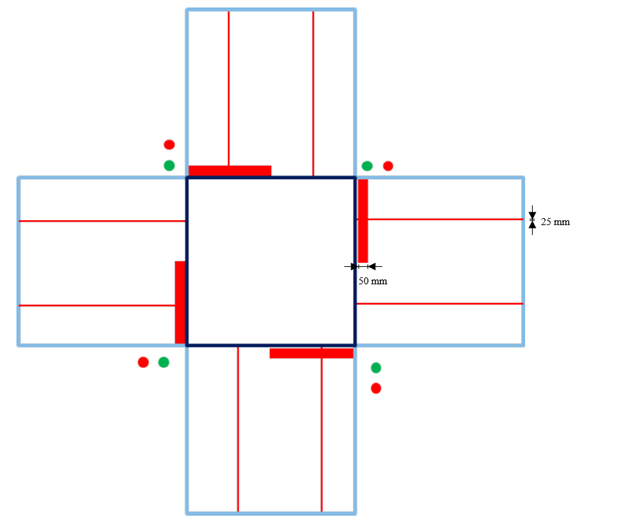
\includegraphics[width=.6\textwidth]{volglijnenEnStoplijnen}
	\caption{Kruispunt}
	\label{fig:plattegrond}
\end{figure}

Om een botsing te voorkomen, moet het autootje voorgaande wagens kunnen detecteren en tijdig stoppen wanneer deze te dichtbij komen. Als de wagen achteraan wordt aangereden, is het niet in fout. Dit impliceert dat enkel voorliggers een probleem kunnen vormen. Om dit op te lossen moet het wagentje uitgerust zijn met een afstandssensor. Deze sensor detecteert voorliggers en verzendt vervolgens een signaal zodat de motoren vertragen. Er moet dus ook gezorgd worden voor een zo kort mogelijke remafstand. %meer uitleg over de remafstand? 

Verder moet de auto aan een aanvaardbare snelheid voortbewegen. De tandwielmotoren rond de wielen zorgen voor de aandrijving. Daarbij is het belangrijk dat het autootje een beperkte massa heeft, maximaal 500 gram. Dit zal ervoor zorgen dat het op een veilige manier voortbeweegt aan een snelheid van ongeveer 10 cm/s. Hierdoor blijft ook de remafstand beperkt.

Uit veiligheid wil men vanop afstand kunnen ingrijpen wanneer er iets fout loopt, zoals een aanrijding. Dit betekent dat de auto naast het autonoom rijden ook bestuurbaar moet zijn via een computer. 


%Per onderdeel verwijzen voor bibliografie!!!

%- herkennen lijnen: welke soort sensor (bv reflectie voor lijnen)
%- stoplicht: kleurensensor, tot stilstand komen blabla
%- snelheid: massa belangrijk
%- andere wagens detecteren => remafstand, massa belangrijk => stoppen door signaal zodat motoren vertragen
%- op afstand ingrijpen


\subsection{Ontwerpskeuze}
%Zeer specifiek toelichten waarom je elk onderdeel heb gekozen.
\label{Ontwerpskeuze}

\subsubsection{Chassis}
Als eerste wordt het chassis besproken. Voor deze auto wordt een rechthoekige variant gebruikt met als afmetingen 80 mm op 172 mm  \cite{RobotChassisRechthoekigZwart}. 

\begin{figure}[ht] 
	\begin{subfigure}[b]{0.5\linewidth}
		\centering
		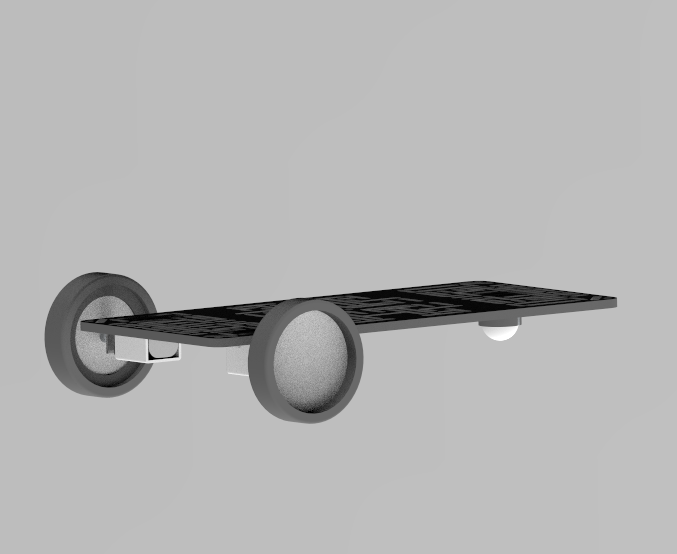
\includegraphics[width=0.75\linewidth]{1chassisaAndrijving} 
		\caption{Chassis met wielen, kogelwiel en motoren} 
		\label{opbouw1} 
		\vspace{4ex}
	\end{subfigure}%% 
	\begin{subfigure}[b]{0.5\linewidth}
		\centering
		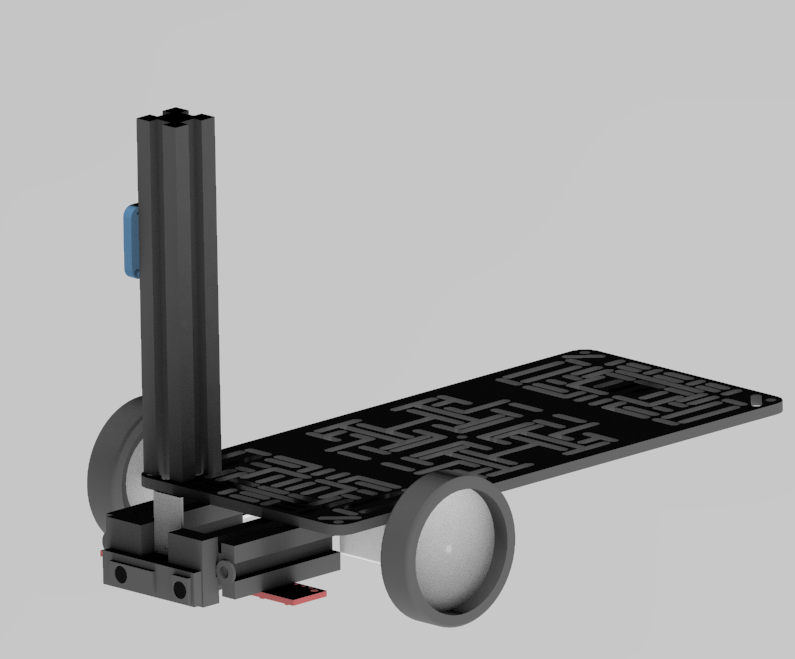
\includegraphics[width=0.75\linewidth]{2sensoren} 
		\caption{Chassis met wielen, kogelwiel, motoren en sensoren} 
		\label{opbouw2} 
		\vspace{4ex}
	\end{subfigure} 
	\begin{subfigure}[b]{0.5\linewidth}
		\centering
		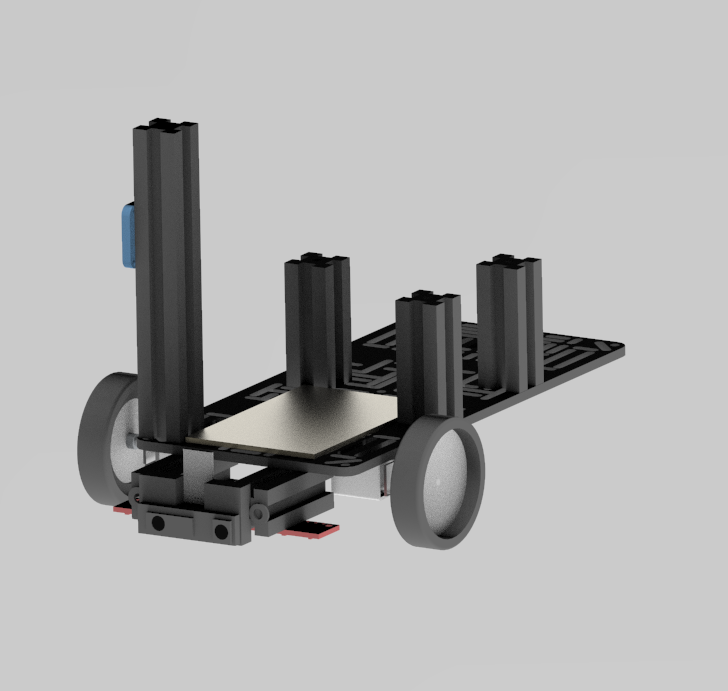
\includegraphics[width=0.75\linewidth]{3voorlaatste} 
		\caption{Chassis met wielen, kogelwiel, motoren, sensoren en makerbeams} 
		\label{opbouw3} 
	\end{subfigure}%%
	\begin{subfigure}[b]{0.5\linewidth}
		\centering
		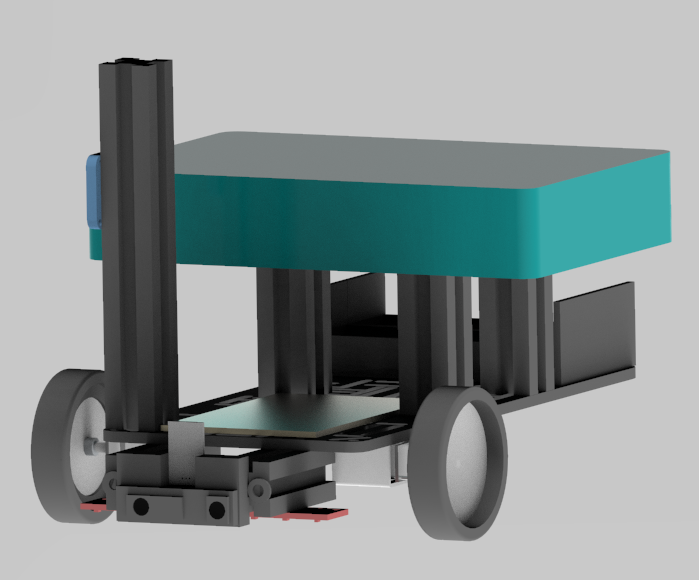
\includegraphics[width=0.75\linewidth]{4Volledig} 
		\caption{De afgewerkte auto} 
		\label{opbouw4} 
	\end{subfigure} 
	\caption{opbouw van de wagen}
	\label{opbouwvanwagen} 
\end{figure}

Deze is handig in gebruik wegens de verscheidene vormen van de groeven. %groottes of vormen?
Bovendien is de rechthoekige vorm zeer gemakkelijk om alle componenten van de auto vast te hechten. Een rond chassis is hiervoor minder geschikt \cite{RobotChassis}. Ook zijn er in dit laatste chassis, groeven aanwezig voor de wielen. Dit impliceert dat er minder ruimte is om andere onderdelen te assembleren op het onderstel. %nadeel nog vermelden over onze 
%motordrivers die er niet aan gesoldeerd konden worden?
\label{Chassis}

\subsubsection{Wielen}
Een goede keuze voor de wielen zijn die met een diameter en dikte van respectievelijk 42 mm en 19 mm.
Figuur \ref{fig:wiel} geeft een idee hoe ze eruit zien.

\begin{figure}
	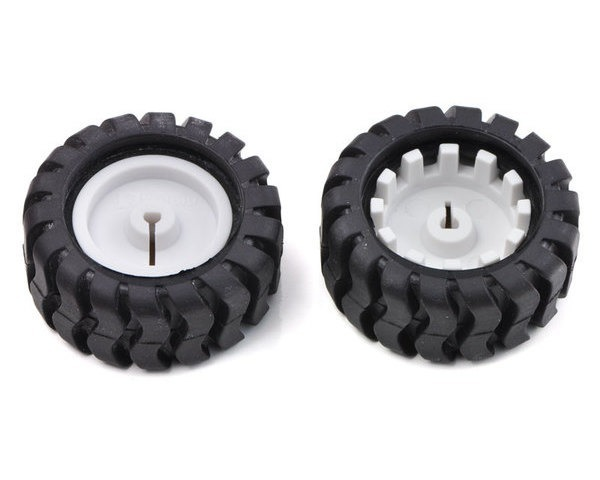
\includegraphics[width=0.5\textwidth]{wielen}
	\centering
	\caption{Wiel met diameter 42 mm en dikte 19 mm} 
	\cite{Wiel42x19mm}.
	\label{fig:wiel}
\end{figure}

De dikte van dit wiel zorgt voor voldoende grip. Bij dunnere banden is er minder grip. Dit zou ervoor kunnen zorgen dat de auto niet snel genoeg kan remmen bij obstakels en stoplijnen \cite{Banden}.  
Daarnaast is de diameter evenredig met de versnelling en de nodige kracht. Een kleiner wiel impliceert een kleinere kracht en een kleine versnelling. Een groot wiel daarentegen levert een grote versnelling maar heeft een grote kracht nodig. Het is dus belangrijk dat de middenweg wordt genomen om een goede snelheid te behalen zonder al te veel moeite.    

De auto van dit project is een driewieler. Dit heeft enkele voordelen. Eerst en vooral is dit eenvoudiger om te draaien. Bij een vierwieler zijn er twee vaste punten. Hierdoor ontstaat er meer wrijving waardoor de auto minder vlot kan draaien. Daardoor is het dus gemakkelijker een driewieler te laten afslaan. Deze heeft bij het afslaan maar één vast punt waarrond de andere wielen draaien. 
Ten tweede reduceert een driewieler de kosten van het project een klein beetje. Een vierde wiel is niet noodzakelijk om aan te schaffen. Op deze manier is er nog een kleine marge in het budget voor eventuele wijzigingen tijdens het project. Als derde wiel voor de auto kiest men voor een kogelwiel. Dit wiel biedt als voordeel flexibeler te zijn in draaibewegingen.  
\label{Wielen}


\subsubsection{Motoren}
Aansluitend spelen de tandwielmotoren ook een belangrijke rol. Motoren met een groot tandwiel starten zeer gemakkelijk maar behalen geen al te grote snelheid. Kleine tandwielen hebben dan weer de omgekeerde eigenschap. Het is dus van belang dat er een tandwielen worden gebruikt met een gemiddelde grootte namelijk de motor met verhouding 50:1. Niet alleen de grootte speelt een rol, maar ook de kracht van de motor. Hiervoor wordt het best gekozen voor de "High Power" (HP). Deze motoren hebben een grote efficiëntie. 

Een bijkomend voordeel is het gewicht dat slechts 9,5 gram bedraagt \cite{MicroMetalGearMotor50:1HP}. %Erbij zetten dat het ook een groter vermogen heeft?
Hoe minder de onderdelen wegen, hoe minder kracht je nodig hebt om de auto te laten rijden. 

Door het gebruik van deze motoren is er nood aan motorbeugels zodat de ze aan het chassis  vastgemaakt kunnen worden. Aangezien de motoren een breedte van 12 mm en een hoogte van 10 mm hebben, is het logisch dat de beugels met afmetingen 12 mm op 10 mm worden genomen \cite{MicroMetalGearMotorBeugel}.
Verder is een dubbele aandrijfmotor essentieel om de tandwielmotoren met de microcontroller te verbinden. In dit project wordt gekozen voor de Dual Drive DRV8833 \cite{DualDriveDRV8833}. 
\label{Motoren}


\subsubsection{Microcontroller}
De microcontroller is cruciaal voor de werking van de auto. Het zorgt ervoor dat het autootje de taken correct uitvoert. De keuze van de microcontroller gaat in dit project naar NI MyRIO in plaats van Raspberry Pi \cite{nimyrio},\cite{RaspberryPi}.
Dit is omdat deze zowel met analoge als digitale signalen kan werken. 
%Dit heeft enkele gevolgen. 
%Eerst en vooral hebben de inputs de mogelijkheid om een digitaal of een analoog signaal door te geven. 
Bij Raspberry Pi zijn er enkel digitale inputs beschikbaar. Dit heeft implicaties voor de keuze van de sensoren, waarvoor ik verwijs naar het onderdeel over sensoren in \ref{Sensoren}.
Daaruit volgt dat alles in LabVIEW geprogrammeerd wordt.
%Ten tweede zal alles in LabVIEW worden geprogrammeerd.
Deze software en microcontroller zijn ervoor gemaakt om samen te werken. Dit biedt veel voordelen tijdens de implementatie. In sectie \ref{Softwareontwerp} wordt hier dieper op ingegaan. %verwijzing nog aanpassen want Sarah ging dat stukje veranderen.
Daarnaast heeft dit ook invloed op de keuze van het chassis. Achteraf viel het op dat de microcontroller niet paste op het chassis waardoor men het heeft vastgemaakt met makerbeams.
%Waarom voor deze microcontroller gekozen: prijs en deze kan met analoge signalen

\label{Microcontroller}

\subsubsection{Sensoren} \label{Sensoren}
Zoals al aangehaald is, wordt in dit ontwerp gewerkt met een reflectiesensor en een afstandssensor. Er bestaan twee soorten, namelijk sensoren met digitale output en met analoge output. Zoals hierboven verteld is, kunnen beiden gebruikt worden met de NI MyRIO. De analoge sensoren geven meer info dan de digitale. De digitale kunnen maar één of twee signalen doorgeven aan de microcontroller namelijk nul of een. Ofwel staat de sensor aan ofwel uit. De analoge sensoren geven analoge signalen. Dit soort signaal kan alle waarden aannemen, in tegenstelling tot een digitaal signaal. Langs de andere kant zorgen de analoge sensoren voor meer programmeerwerk \cite{DigitaalOfAnaloog}. Voor dit project is het beter dat de informatieoverdracht tussen sensor en microcontroller vlot verloopt met behulp van echte waarden. Bij keuze van een analoge sensor is dit dus voldaan. %echte waarden nog wat uitleggen wat ermee bedoeld wordt. experimentele waarden?
De reflectiesensor zal onderaan de auto, dichtbij de grond geplaatst worden zodat de lijnen op het juiste moment zullen herkend worden. Ook is de reflectiesensor iets breder dan de volglijn. Zo zal het vanaf de auto bij een stoplijn komt, andere waarden binnenkrijgen.

~

Ook om de kleuren groen en rood te herkennen, is er nood aan een kleurensensor of camera. Er is keuze tussen een Raspberry Pi-camera, webcam en kleurensensor voor het interpreteren van de stoplichten. In dit ontwerp wordt gekozen voor de kleurensensor. Deze is compatibel met de NI MyRIO en weegt maar 3,23 gram \cite{Webcam,TCS34725KleurSensorBOB}. Bovendien weegt de webcam 223,6 gram. Hoe minder de wagen weegt, hoe stabieler het is en hoe minder kracht het nodig heeft om een bepaalde snelheid te kunnen halen. De Raspberry Pi-camera is enkel bruikbaar met een Raspberry Pi als microcontroller. Aangezien in dit model wordt gewerkt met een NI MyRIO, is dit dus geen optie \cite{RPi-camera}. Samengevat: de kleurensensor heeft als voordeel dat het zeer licht is en compatibel is met de NI MyRIO-microcontroller. % 2 keer is? 



\subsubsection{LED-lampjes}\label{LED-lampjes}
Als extra optie kozen we om LED's te voorzien, dit zorgt ervoor dat omstaanders kunnen waarnemen welke richting het wagentje zal uitgaan. Daarnaast leek het ons ook een haalbare extra opdracht. Eerst dachten we eraan om servomotoren te gebruiken maar deze waren schaars en ingewikkeld te modelleren en programmeren waardoor er risico zou zijn dat het wagentje niet juist werkt.
%Gear-motor: niet 100, want anders veel toeren, maar te weinig kracht (50 omgekeerd)


\subsection{Assemblage}\label{Assemblage}
%titel nog aan te passen
%Alles op elkaar zetten, 3D-modellen?
%NOG DOEN
Voordat het autootje fysiek geassembleerd wordt, werd dit eerst via de computer gedaan. Aan de hand van de reeds gemaakte 3D-modellen, werd een 3D-model van het autootje gemaakt. Doordat de apparte onderdelen van het autootje al af waren, moesten die enkel nog samengevoegd worden. Het 3D-model zie je in figuren \ref{opbouw1}, \ref{opbouw2}, \ref{opbouw3} en \ref{opbouw4}.
Door dit model was het gemakkelijker om de wagen in elkaar te zetten omdat er zo naar iets toegewerkt kon worden. Ook was hierdoor de plaatsing van de onderdelen zichtbaar.%Deze zin is nogsteeds niet mooi maar ik weet niet goe hoe het anders te zeggen.
Het ontwerp start bij het chassis. hierbij worden dan de motoren met wielen aan de onderkant geplaatst. Ook het kogelwiel wordt bevestigd aan de onderkant. Helemaal vooraan worden twee steunpalen bevestigd. De reflectiesensor wordt onder de steunpaal vast gemaakt. Ook aan de voorkant wordt de afstandsensor geplaatst. Deze sensor wordt niet aan de onderkant vastgemaakt, maar aan de voorkant van deze twee palen. Aan de rechterzijkant wordt nog een grotere paal geplaast, zodat de kleursensor op een hoogte van 7.5 cm de stoplichten kan lezen. Net achter de steunpaal wordt de {\it dual drive motor} op de printplaat gesoldeerd. Op het midden van het chassis ondersteunen drie kleinere palen de microcontroller. 






\section{Softwareontwerp}\label{Softwareontwerp}

Om te kunnen implementeren is het belangrijk om informatie in te winnen via opzoekingswerk. Het is dan ook cruciaal dat er specifieker wordt gezocht hoe het materiaal best gebruikt kan worden.
%bron myrio nog vermelden
Dit is nuttig om de communicatie tussen de sensoren en de NI MyRIO-controller te begrijpen. Ook de spanning dat nodig is om de sensoren te laten te werken is belangrijk. Zo zijn er enkele poorten die precies 5 volt leveren. Dit is perfect, aangezien dit compatibel is met het spanningsverschil van de sensoren. Vervolgens kan het elektrisch circuit opgesteld worden. Dit is handig om te weten welke onderdelen er met elkaar worden verbonden. Eenmaal dit in orde is, kan het programmeerwerk beginnen.
%Laatste twee zinnen nog aan te passen.

Voor het schrijven van stukjes code, is het ten sterkste aangeraden om over de onderdelen van de auto te beschikken opdat de fragmenten van de code kunnen worden uitgetest. In de subsectie die volgt wordt een korte analyse gegeven van de observaties die volgen uit kleine experimenten. Om de testen mogelijk te maken, moet er eerst contact worden gemaakt tussen een computer en de microcontroller. Dit kan gerealiseerd worden met de ´LED´ functie in LabVIEW. Eenmaal er connectie is, branden de lampjes op de microcontroller en kunnen de experimenten van start gaan.


\subsection{Experimenten}
\subsubsection{Signalen ontvangen en versturen}
Er zijn vijf experimenten gebeurd. Er zijn twee experimenten geweest om de communicatie met de microcontroller te testen. 
Bij het eerste experiment werden de lampjes van de microcontroller aan en uitgezet met een schakelaar in LabVIEW.
Het andere experiment, was om een signaal terug te krijgen van de microcontroller.
Er werden twee poorten van de my Rio met elkaar verbonden en als de microcontroller gekanteld werd, moest een signaal verstuurd worden van de ene poort naar de andere.
Er is nu communicatie mogelijk want het kan signalen versturen en ontvangen.


\subsubsection{Sensoren}

Vervolgens werden er drie experimenten uitgevoerd om de waarden van de sensoren te begrijpen.
Als men niet weet wat een bepaalde waarde betekent, kan men het programma niet schrijven.
Bij de reflectiesensor werden de waarden van wit, grijs en zwart getest. 
Voor zwart werden waarden tussen drie en vier terug gegeven.  
Voor de kleursensor werd er getest met het rood en groen van de verkeerslichten.
De sensor detecteerde nauwelijks groene waardes, dus besloten we om ons enkel te baseren op de rode waardes die we van de kleursensor verkregen.
Voor de afstandssensor werd een boek gehouden en deze verschoof zodat de waarden op verschillende afstanden gekend was.
Er werd een piekwaarde van drie teruggeven bij een afstand van 10 cm. 
Deze waarden en resultaten werden gebruikt om het eind programma te generen.

%Met behulp van voorbeeldprogramma's is het mogelijk om de gekregen data die van de sensoren te interpreteren. Zo is er een idee met welke waarden er moet gewerkt worden in het definitief programma. 

%Een eerste experiment is met de reflectiesensor. Deze sensor werkt met een programma dat de acht waarden teruggeeft. 
%Een van de vereisten voor het autootje is een lichte en donkere kleur te onderscheiden. Om te weten welke waarden de sensor geeft, kan dit worden getest met een wit papier, de zwarte voorkant van een laptop en een grijs tafelblad. Bij het papier wordt een waarde dichtbij 1 verkregen terwijl bij het donkere spectrum waarden tussen 4 en 4,5. %en de tafel?
%Door het experimentje is er nu geweten welke waarden er moeten gebruikt worden om de lijn op de grond te kunnen volgen.
% !!!!!!!! Eventueel hetgene hieronder weglaten?? Is dit noodzakelijk voor het verslag????
% We hebben het aantal waarden dat we krijgen per seconde wat vermindert van 1000 naar 100 om op die manier stabielere inputs te krijgen. Anders was het moeilijk om die waarden te lezen.

%Het volgende experiment is met de afstandssensor. Bij deze test wordt een voorwerp eerst ver van de sensor gehouden en dan dichterbij. Bij afstanden kleiner dan 80 cm worden lage waarden bekomen zoals 0,1. Afstanden groter dan 80 cm geven een negatieve waarde. Wanneer de afstand echter op een tiental cm van de sensor verwijderd is, wordt een maximale waarde van 3 verkregen. Eenmaal de lengte tussen de afstandssensor en het voorwerp kleiner is dan 10 cm, zakt de geleidelijk aan naar 2. De conclusie van deze test: voor de afstandssensor zullen de waarden twee en drie moeten gebruikt worden.

\subsection{Programma's}\label{definitieve programma's}
% Define block styles
\tikzstyle{decision} = [diamond, draw, fill=orange!20, text width=4.5em, text badly centered, node distance=3cm, inner sep=0pt]
\tikzstyle{block} = [rectangle, draw, fill=blue!20, text width=5em, text centered, rounded corners, minimum height=4em]
\tikzstyle{line} = [draw, -latex']
\tikzstyle{cloud} = [draw, ellipse,fill=red!20, node distance=3cm,
minimum height=2em]


Om het programma volledig te begrijpen, zal alles stap voor stap worden uitgelegd met behulp van verscheidene korte flowcharts. \\

In schema \ref{programmaBegin} wordt de opsplitsing tussen de manuele en automatische besturing toegelicht. Bij dit programma is het belangrijk om op te merken dat bij een overschakeling naar de manuele besturing de waarden 0, 1 en 2 telkens automatisch worden gereset opdat er steeds manueel kan gereden worden. %nog aan te passen.
Zodra de overschakeling naar de automatische besturing gebeurt, wordt er telkens een waarde verstuurd 0, 1, en 2. Deze waarden worden verder verduidelijkt in aparte flowchart respectievelijk \ref{reflectiesensorValueZero}, \ref{kleursensorValueOne} en % nog te maken.
In het schema wordt ook gebruik gemaakt van de Engelse afkortingen PWM en RGB. De eerste afkorting staat voor Puls width modulation of in het Nederlands pulsbreedtemodulatie. Dit is een techniek waarbij vaste frequentie pulsen in een soort van blokstructuur worden uitgezonden.%\cite{bibid}
De tweede afkorting geeft de kleuren aan die de kleurensensor kan waarnemen namelijk rood, groen en blauw.
\\
\begin{figure}
	\label{programmaBegin}
	\centering
	\begin{tikzpicture}[node distance = 2.5cm, auto]
		%place
		\node [cloud](start){start};
		\node [block, below of= start](sensor data){Sensor data};
		\node [decision, below of= sensor data](manueel){Manuele besturing aan?};
		\node [block, below right of= manueel](auto){Welke sequentie? (default = 0)};
		\node [decision, below left of= manueel](knoppen){Gebruik controleknoppen};
		\node [draw, trapezium, fill=gray!20, trapezium left angle = 65, trapezium right angle = 115, below left of= knoppen](PWM){PWM};
		\node [draw, trapezium, fill=gray!20, trapezium left angle = 65, trapezium right angle = 115, below left of = auto](0){Sequentie 0 \ref{reflectiesensorValueZero}};
		\node [draw, trapezium, fill=gray!20, trapezium left angle = 65, trapezium right angle = 115, below right of = 0](1){Sequentie 1 \ref{kleursensorValueOne}};
		\node [draw, trapezium, fill=gray!20, trapezium left angle = 65, trapezium right angle = 115, below right of = auto](2){Sequentie 2 \ref{sequentie2}};
		% lines
		\path [line] (start) -- (sensor data);
		\path [line] (sensor data) -- (manueel);
		\path [line] (manueel) -- node {nee} (auto);
		\path [line] (manueel) -- node {ja} (knoppen);
		\path [line] (knoppen) -- (PWM);
		\path [line] (PWM) |- node {nieuwe iteratie}(sensor data);
		\path [line] (auto) -- (0);
		\path [line] (auto) -- (1);
		\path [line] (auto) -- (2);
	\end{tikzpicture}
	\caption{De algemene structuur van het basisprogramma.}
\end{figure}

\begin{figure}
	\label{reflectiesensorValueZero}
	\hspace*{-0.5cm}
	\begin{tikzpicture}[node distance = 3cm, auto]
		%place nodes
		\node [draw, trapezium, fill=gray!20, trapezium left angle = 65, trapezium right angle = 115](0){Sequentie 0};
		\node [block, below of = 0] (begin) {Data reflectiesensor gebruiken};
		\node [decision, below of=begin] (lijn) {Lijn gedetecteerd?};
		\node [draw, trapezium, fill=gray!20, trapezium left angle = 65, trapezium right angle = 115, below right of=lijn] (hervat) {Blijf op sequentie 0};
		\node [decision, below left of=lijn] (welke) {Stoplijn?};
		\node [draw, trapezium, fill=gray!20, trapezium left angle = 65, trapezium right angle = 115, below left of=welke] (stoplijn) {Ga naar sequentie 1 \ref{kleursensorValueOne}};
		\node [block, below right of=welke] (volglijn) {Volg de lijn};
		%place paths
		\path [line] (0) -- (begin);
		\path [line] (begin) -- (lijn);
		\path [line] (lijn) -- node {ja} (welke);
		\path [line] (lijn) -- node {nee} (hervat);
		\path [line] (welke) -- node {ja} (stoplijn);
		\path [line] (welke) -- node {nee} (volglijn);
		\path [line] (volglijn) |- (welke);
		\path [line] (hervat) |- node {nieuwe iteratie} (0);
	\end{tikzpicture}
	\caption{Het basisidee van het programma van de reflectiesensor voor de sequentie 0.}
\end{figure}

\begin{figure}
	\label{kleursensorValueOne}
	\centering
	\begin{tikzpicture}[node distance = 3cm, auto]
		%place nodes
		\node [draw, trapezium, fill=gray!20, trapezium left angle = 65, trapezium right angle = 115](1){Sequentie 1};
		\node [decision, below of= 1] (Rood) {Was het rood?};
		\node [decision, below left of=Rood] (Groen) {Groen?};
		\node [decision, below right of=Rood] (controle) {Rood?};
		\node [draw, trapezium, fill=gray!20, trapezium left angle = 65, trapezium right angle = 115, below right of=Groen] (volgende) {Ga naar sequentie 2 \ref{sequentie2}};
		\node [draw, trapezium, fill=gray!20, trapezium left angle = 65, trapezium right angle = 115, below left of=Groen] (opnieuw) {Blijf op sequentie 1};
		\node [block, below right of=controle] (waarde) {Onthoud de waarde};
		%\node [draw, trapezium, fill=gray!20, trapezium left angle = 65, trapezium right angle = 115, below of=waarde] (herbegin) {Waarde 1};
		%place paths
		\path [line] (1) -- (Rood);
		\path [line] (Rood) -- node {ja} (Groen);
		\path [line] (Rood) -- node {nee} (controle);
		\path [line] (Groen) -- node {ja} (volgende);
		\path [line] (Groen) -- node {nee} (opnieuw);
		\path [line] (controle) -- (waarde);
		%\path [line] (waarde) -- (herbegin);
		\path [line] (waarde) |- node {controle}(1);
		\path [line] (opnieuw) |- node {controle}(1);
	\end{tikzpicture}
	\caption{Het basisidee van het programma van de kleurensensor met behulp van de sequentie 1.}
\end{figure}

Nog een interessante opmerking over onderdeel \ref{sequentie2} van het basisprogramma. TO DO: nog verder schrijven

\begin{figure}
	\hspace*{-2.5cm}
	\label{sequentie2}
	\begin{tikzpicture}[node distance = 4.5cm, auto]
		\node [draw, trapezium, fill=gray!20, trapezium left angle = 65, trapezium right angle = 115](2){Sequentie 2};
		\node [decision, below of = 2](draaien){Draaien?};
		\node [block, below of= draaien](instellen){PWM instellen};
		\node [decision, below right of= instellen](iteraties){25 iteraties zonder lijn?};
		\node [decision, right of= iteraties](JaGevonden){Lijn gevonden?};
		\node [decision, below left of= iteraties](NeeGevonden){Lijn gevonden?};
		\node [draw, trapezium, fill=gray!20, trapezium left angle = 65, trapezium right angle = 115, below right of=JaGevonden] (waarde0) {Ga naar sequentie 0 \ref{reflectiesensorValueZero}};
		\node [draw, trapezium, fill=gray!20, trapezium left angle = 65, trapezium right angle = 115, above right of=JaGevonden] (opnieuw) {Blijf op sequentie 2};
		\node [draw, trapezium, fill=gray!20, trapezium left angle = 65, trapezium right angle = 115, below left of=NeeGevonden](optellen){Telling van de iteratie +1};
		\node [draw, trapezium, fill=gray!20, trapezium left angle = 65, trapezium right angle = 115, below right of=NeeGevonden](resetten){Reset de telling van de iteratie};
		\node [block, above right of= draaien](rechtdoor){Rechtdoor rijden};
		\node [block, right of= rechtdoor](uit){LED's uit};
		\node [decision, below right of= draaien](rechts?){Rechts?};
		\node [block, above right of= rechts?](linker){Linker rictingsaanwijzer aan};
		\node [block, right of= rechts?](rechter){Rechter richtingsaanwijzer aan};
		% setting arrows
		\path [line] (2) -- (draaien);
		\path [line, dashed] (draaien) -- (instellen);
		\path [line] (instellen) -- (iteraties);
		\path [line] (iteraties) -- node {ja} (JaGevonden);
		\path [line] (iteraties) -- node {nee} (NeeGevonden);
		\path [line] (JaGevonden) -- node {ja} (waarde0);
		\path [line] (JaGevonden) -- node {nee} (opnieuw);
		\path [line] (NeeGevonden) -- node {ja} (resetten);
		\path [line] (NeeGevonden) -- node {nee} (optellen);
		\path [line] (draaien) -- node {nee} (rechtdoor);
		\path [line] (rechtdoor) -- (uit);
		\path [line] (draaien) -- node {ja} (rechts?);
		\path [line] (rechts?) -- node {ja} (rechter);
		\path [line] (rechts?) -- node {nee} (linker);
	\end{tikzpicture}
	\caption{In een notendop het programma om het autootje te laten draaien.}
\end{figure}

Naast het basisprogramma is de implementering van de afstandssensor nuttig om beter te begrijpen. Dit wordt verduidelijkt met flowchart \ref{afstandssensor}.
\\
TO DO: juiste referentie naar de figuren
\\
\begin{figure}
	\label{afstandssensor}
	\centering
	\begin{tikzpicture}[node distance = 3cm, auto]
		% Place nodes
		\node [cloud](start){Start};
		\node [decision, below of=start] (voorligger) {Voorligger?};
		\node [decision, right of=voorligger] (verder) {Dichter dan 20 cm?};
		\node [block, below left of=voorligger,] (rijden) {Auto rijdt};
		\node [decision, right of=verder] (dichtbij) {Dichter dan 10 cm?};
		\node [block, above of=dichtbij] (vertragen) {Vertragen};
		\node [block, below right of=dichtbij] (stoppen) {Auto stopt};
		\node [cloud, below of=stoppen] (einde) {Stop};
		% Draw edges 	
		\path [line] (start) -- (voorligger);
		\path [line] (voorligger) -- node {ja} (verder);
		\path [line] (voorligger) -- node {nee} (rijden);
		\path [line] (verder) |- node {nee} (rijden);
		\path [line] (rijden) |- (start); 
		\path [line] (verder) -- node {ja} (dichtbij);
		\path [line] (dichtbij) -- node {nee} (vertragen);
		\path [line] (vertragen) -- (verder);
		\path [line] (dichtbij) -- node {ja} (stoppen);
		\path [line] (stoppen) -- (einde);
	\end{tikzpicture}
	\caption{Het basisidee van het programma van de afstandssensor.}
\end{figure}

TO DO: hoe het draaien precies verloopt, hoe de wielen draaien



\section{Discussie} %discussiesectie 
\subsection{Resultaten demo}  % Dit deel geschreven door Dieter Demuynck 
Er wordt een demonstratie gehouden om de functionaliteit van het autootje te testen. Dit is nuttig om te kijken of het inderdaad doet wat er gevraagd wordt en hoe efficiënt het werkt.

% Algemene problemen.
Er werd vastgesteld dat de auto soms van de lijn reed. Daarnaast had het veel moeite met te draaien op een correcte manier. Bovendien reed het soms door het rood. Dit heeft hoogstwaarschijnlijk te maken met de gebruikte componenten en de algemene bouw van de wagen. Het wagentje kon wel snel genoeg rijden om de uitgestippelde weg op een redelijke snelheid af te leggen.

% Problemen met motoren
Eén van de oorzaken, bleek dat de motoren niet even snel en gelijkmatig draaiden. Ook hadden ze soms niet genoeg kracht om vooruit te rijden. Dit kwam vooral voor wanneer de wagen op één wiel probeert te draaien, bijvoorbeeld in bochten. Mogelijks is dit te wijten aan te veel wrijving tussen het kogelwiel en de grond, en/of te weinig wrijving tussen de wielen en de grond. Om toch die ongelijkmatigheid te beperken, werden er twee waarden ingevoerd om de snelheid van de motor die het snelste draaide te verlagen. Op die manier moesten beide motoren niet uitgeschakeld worden opdat de kracht voldoende groot bleef om toch verder te kunnen rijden. Dit zorgde echter voor nieuwe problemen. Zelfs met snelheidsaanpassingen reed de aanvankelijke snelste motor niet altijd even snel als werd ingegeven, zoals tijdens bochten. Hoogstwaarschijnlijk komt dit doordat één wiel meer of minder kracht ondervindt. Ook kan het gebeuren dat er een wiel slipt en geen of te weinig grip heeft. Deze twee redenen zorgden ervoor dat de wagen soms van de lijn afweek, ook al probeerde het toch om zich aan te passen om op de lijn te blijven. Hierdoor was er de noodzaak om veelal tijdens bochten manueel in te grijpen.
%Eerste zin over snelheid motoren niet gelijkmatig staat wat te ver van de uitleg die erbij hoort!

% Problemen met kleurensensor
Zoals eerder aangehaald, reed het autootje soms door een rood licht. De oorzaak hiervan ligt bij het ingewikkelde algoritme van de kleurensensor dat besluit of het groen of rood is. Er is enkel een heel geringe verandering in de rode en groene waarden door de flikkering van het rood of groen licht aan 1 Hz. Deze flikkering is net het probleem bij het opmeten, aangezien er geen flikkering wordt opgemeten bij het rood licht, ook al is het rood. Dit zorgt ervoor dat de auto door rijdt.

% Besluit: Mogelijke oplossingen
Uit de demo kan er besloten worden welke mogelijke verbeteringen en aanpassingen er in de toekomst gemaakt kunnen worden opdat een beter resultaat verkregen wordt. Een eerste verbetering zou kunnen zijn om het zwaartepunt van de auto op de wielen te laten rusten, en minder op het kogelwiel. Een andere mogelijkheid is om meerdere kogelwielen te gebruiken zodat de kracht meer wordt verdeeld. Daarnaast kunnen er ook krachtigere wielen gebruikt worden. Er zou ook eventueel overwegen kunnen worden om een camera te gebruiken, samen met een passend algoritme, om de verkeerslichten beter te interpreteren.
\\

\subsection{Financiële kant} 
In het financieel rapport \ref{financieel rapport} krijgt men een beeld van wat er is aangekocht en hoeveel eenheden hieraan zijn besteed.  

In dit project kreeg elke groep 3500 eenheden om te bieden en onderdelen te bestellen voor de auto. Bij de eerste bestelling werden in totaal 1615 eenheden uitgegeven. Na de bieding, waaraan 1350 eenheden werden gespendeerd, bleven er nog 311 eenheden over.



\section{Besluit}
Het is duidelijk dat er veel opzoekingswerk vereist is. Er moet namelijk gezorgd worden dat alle onderdelen bij elkaar passen: geen te grote wielen, onderdelen die niet te veel wegen… Dit is het belangrijkste onderdeel van het ontwerpproces.\\
Voor het implementeerwerk is er ook heel wat opzoekingswerk vereist. Daarom is het belangrijk dat dit werk tijdig wordt ingepland, zodat men genoeg tijd zal hebben om effectief te programmeren. Eens er begonnen wordt met het programmeren is het ten sterkste aangeraden om over de onderdelen van de auto te beschikken. Zo zal er geëxperimenteerd kunnen worden. Om een beter beeld te krijgen over de programma’s die moeten geïmplementeerd worden, is het handig om vooraf een flowchart te maken. Aan de hand van deze flowcharts zou het haalbaar moeten zijn om het volledig programma uit te schrijven.\\
Om in de toekomst de auto te verbeteren, is het aanbevolen om meer gewicht op de wielen te laten rusten, zodat het kogelwiel achteraan minder wrijving ondervindt. Het gebruik van krachtigere wielen kan hier ook een oplossing bieden. Daarnaast is het misschien beter om een camera te gebruiken voor het interpreteren van een verkeerslicht. Een nadeel hiervan is het bijkomend gewicht. 
Extra tijd voor dit project zou bovendien ook betekenen dat de programma’s meer getest zouden kunnen worden waardoor deze nog verbeterd kunnen worden.


%Samenvatting wat in verslag
%Conclusie: werkte goed of niet
%Future outlook: wat zou je nog doen als je nog weken extra had, verbetering
%future.

\newpage

\appendix
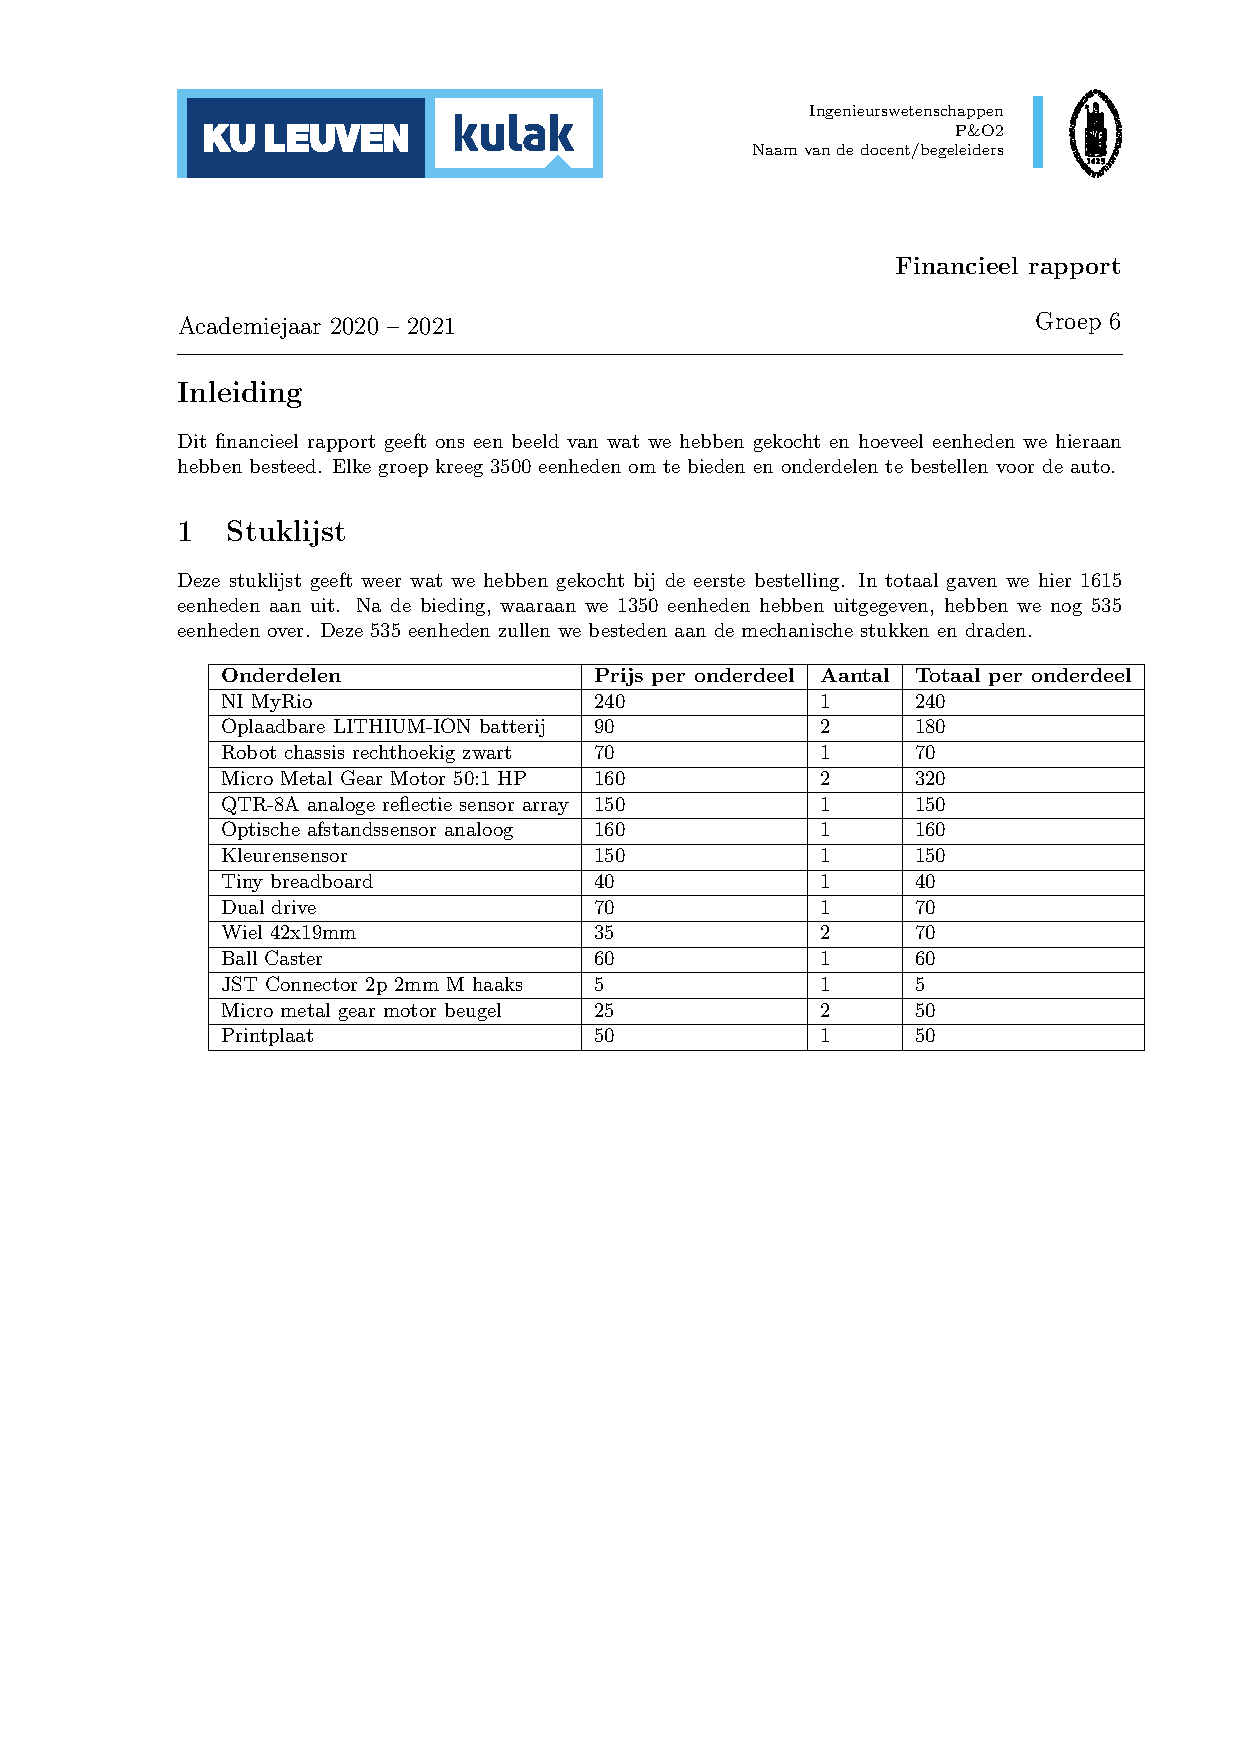
\includepdf{FinancieelRapport.pdf}\label{financieel rapport}
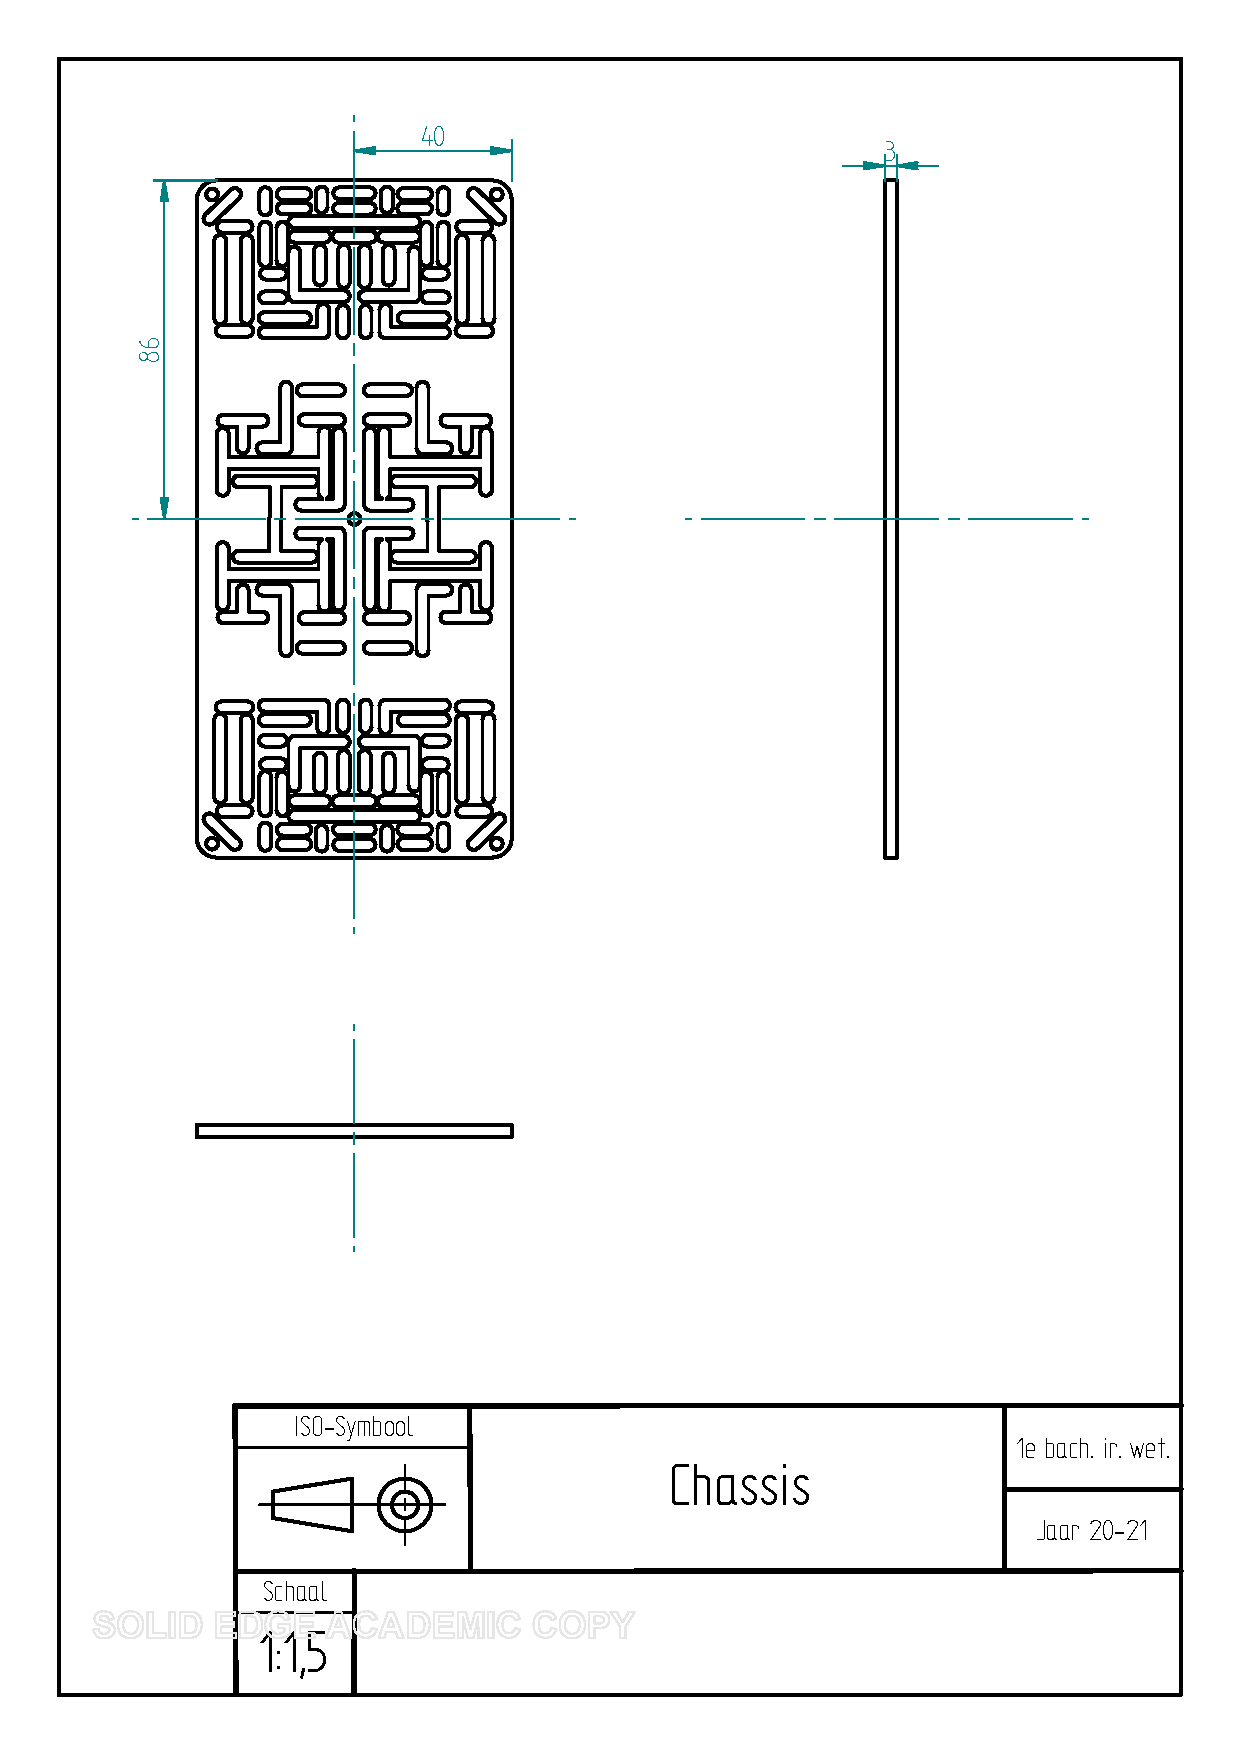
\includepdf{TechnischeTekeningChassis.pdf}\label{TechTekChassis}
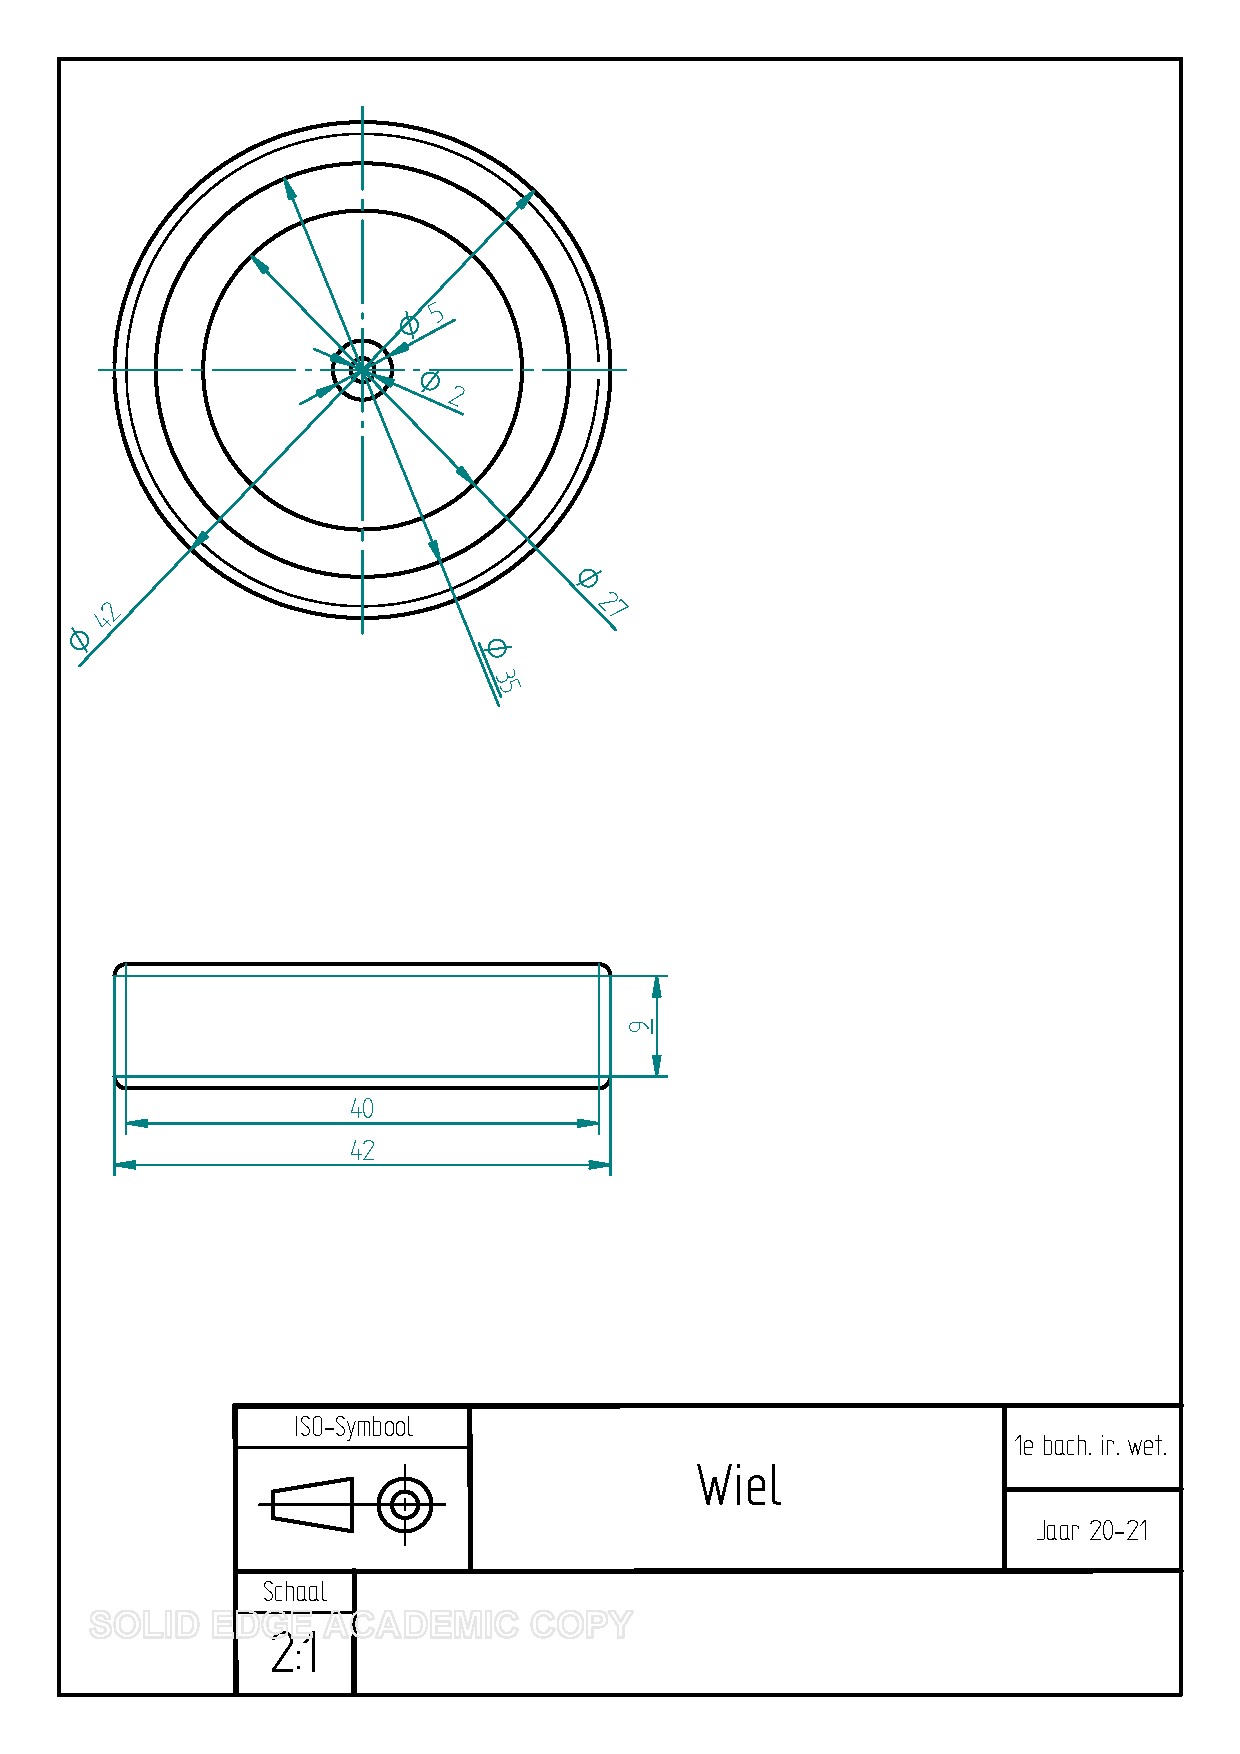
\includepdf{TechnischeTekeningWiel.pdf}\label{TechTekWiel}
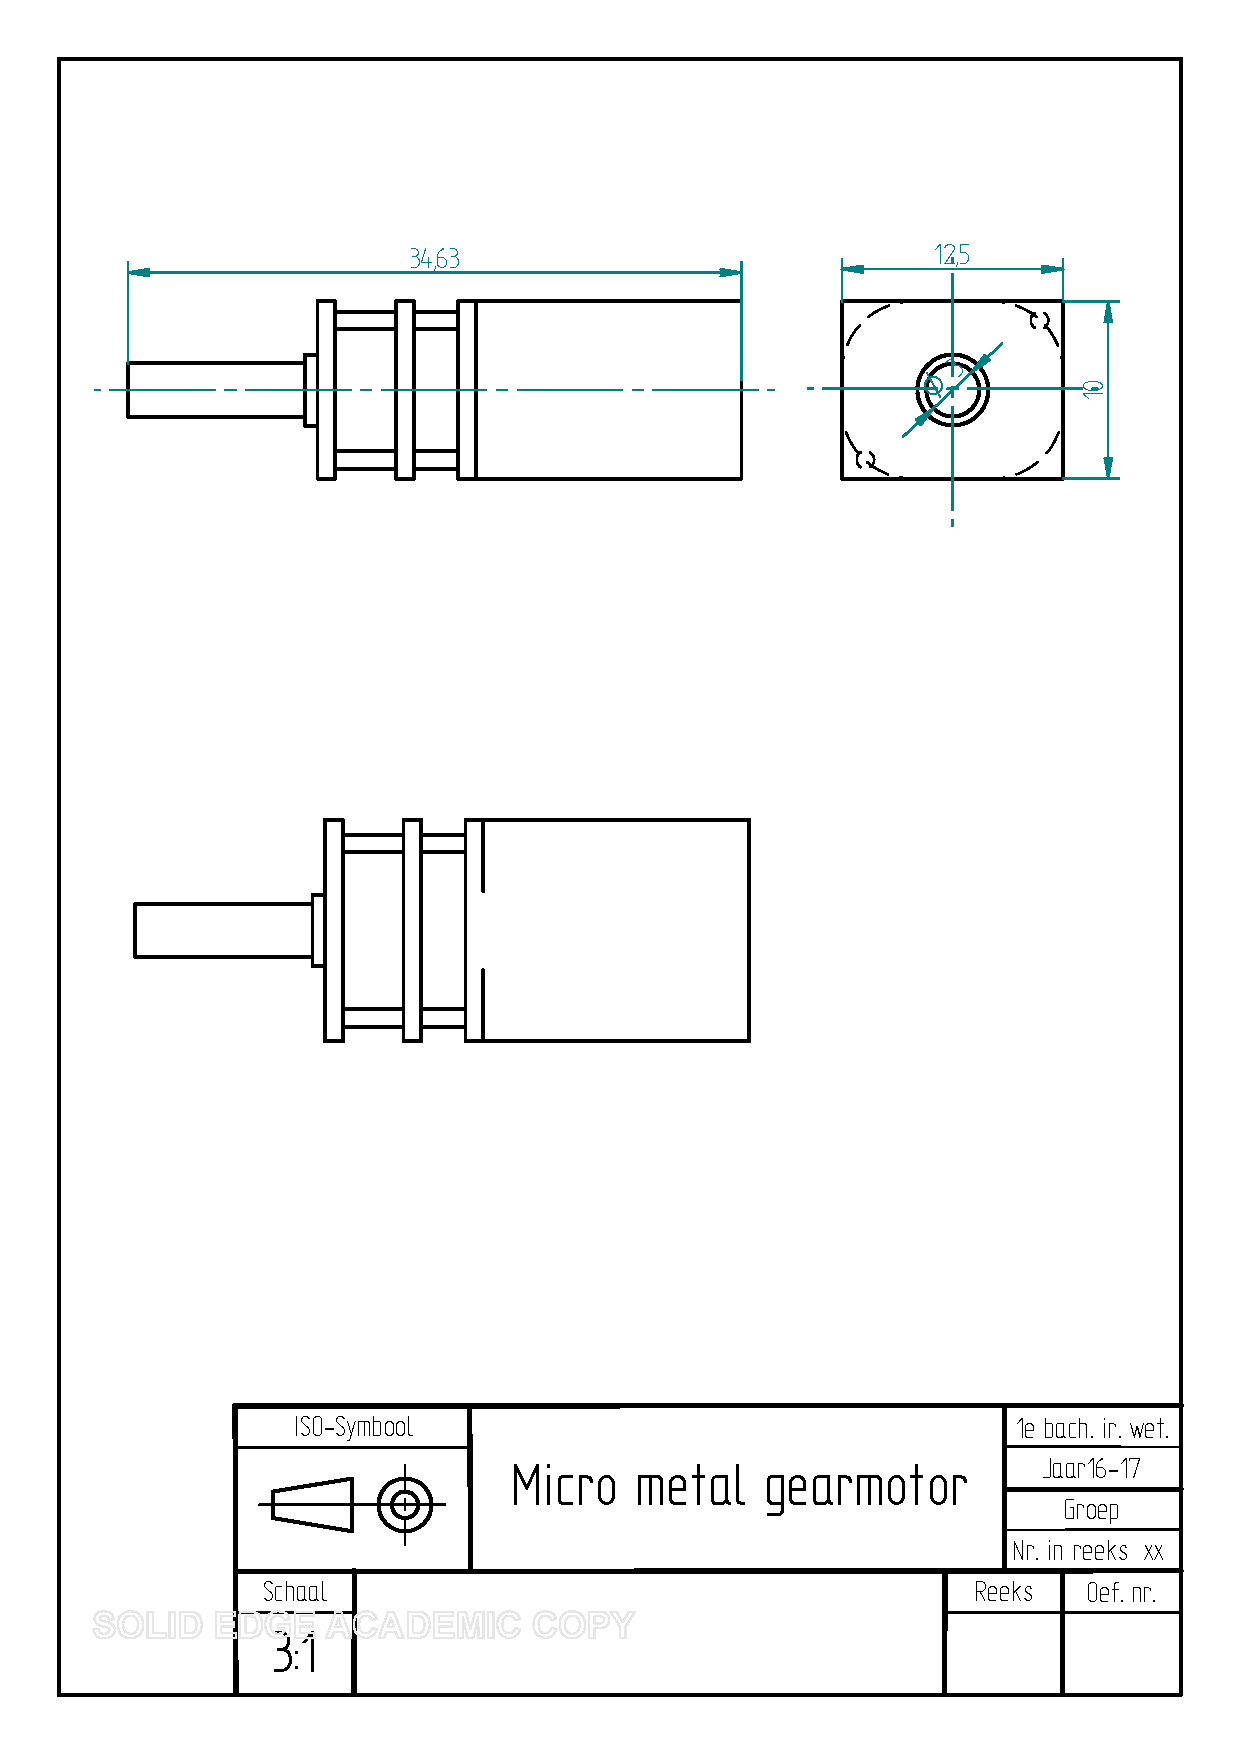
\includepdf{TechnischeTekeningMotor.pdf}\label{TechTekMotor}
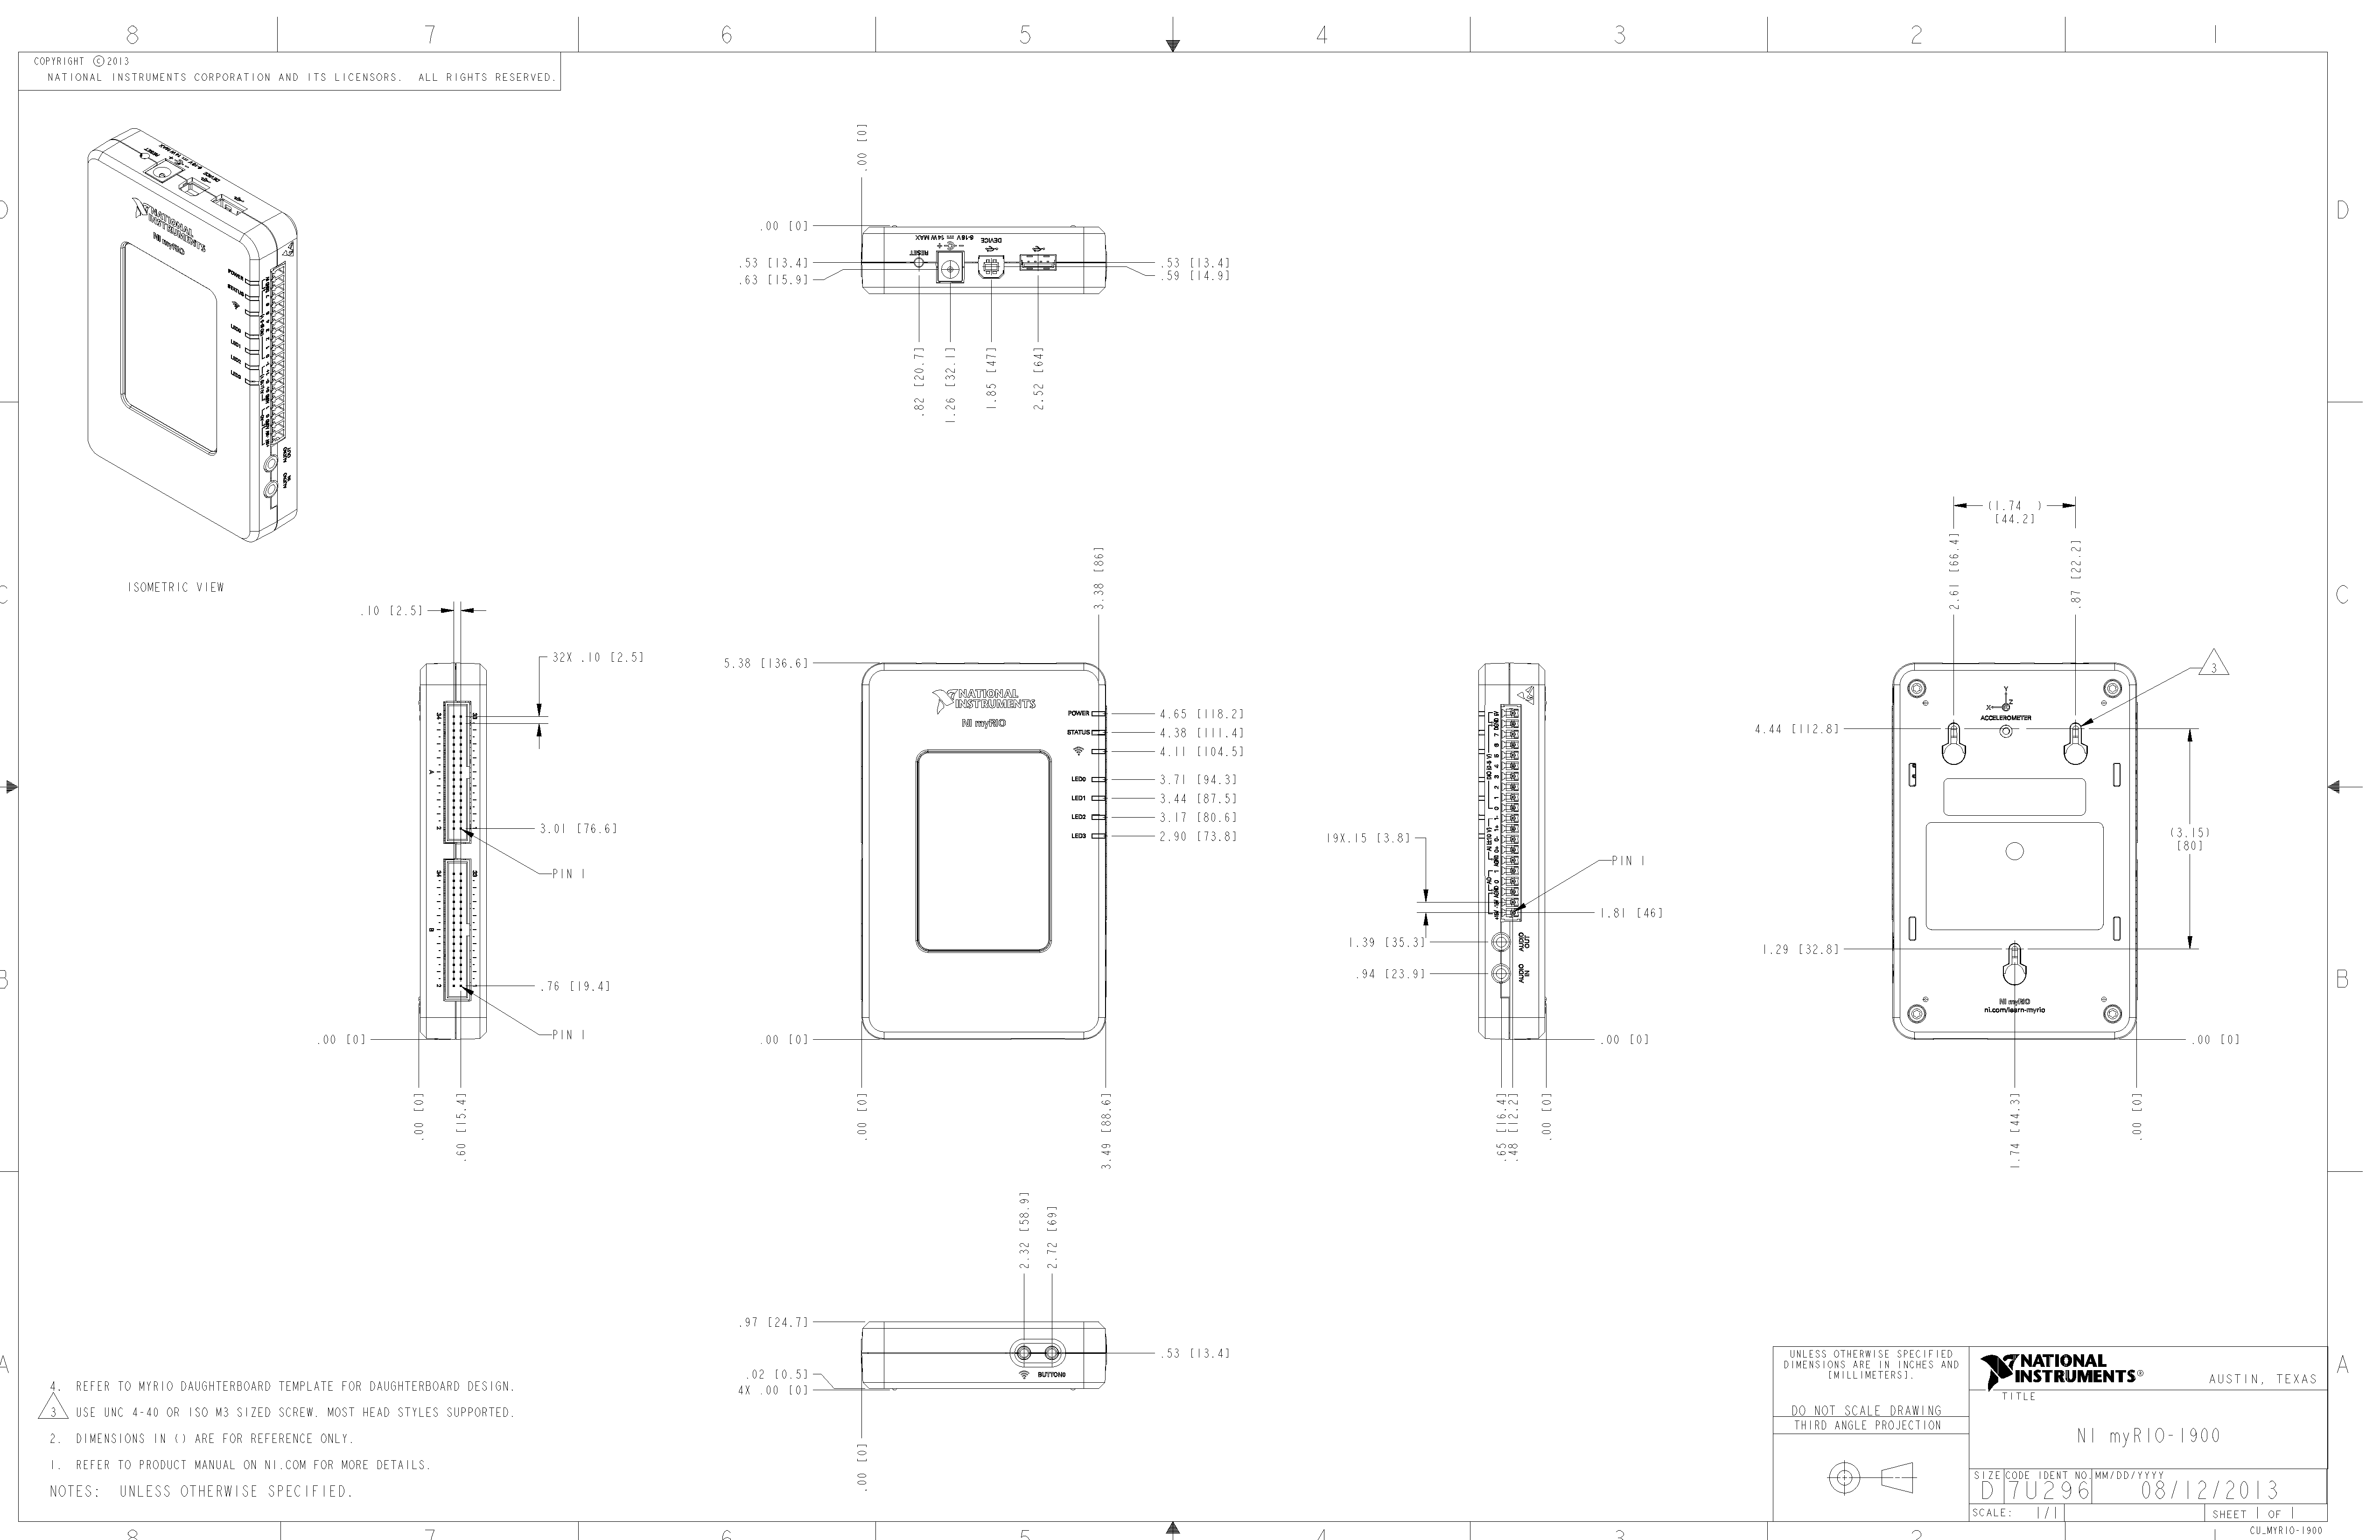
\includepdf{TechnischeTekeningMicrocontroller.pdf}\label{TechTekMicrocontroller}
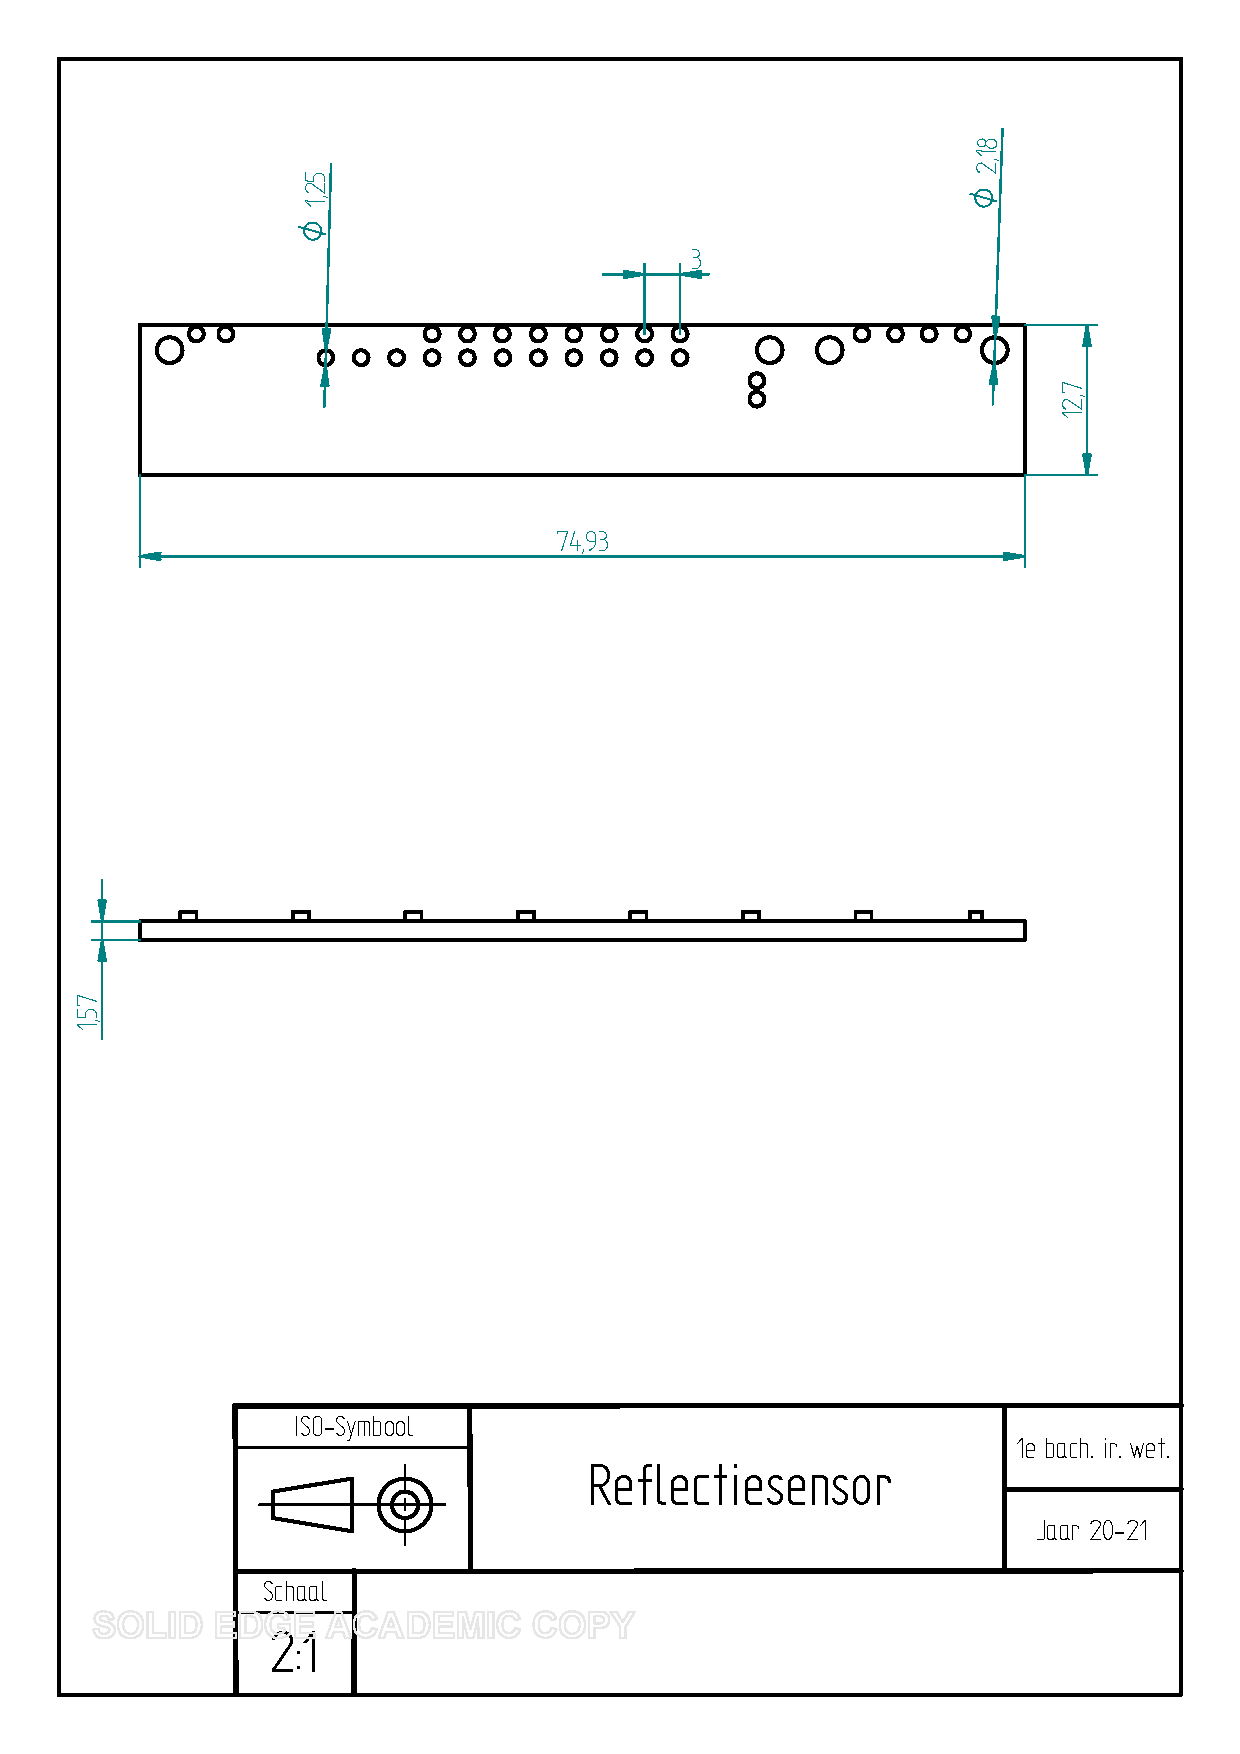
\includepdf{TechnischeTekeningReflectiesensor.pdf}\label{TechTekReflectiesensor}
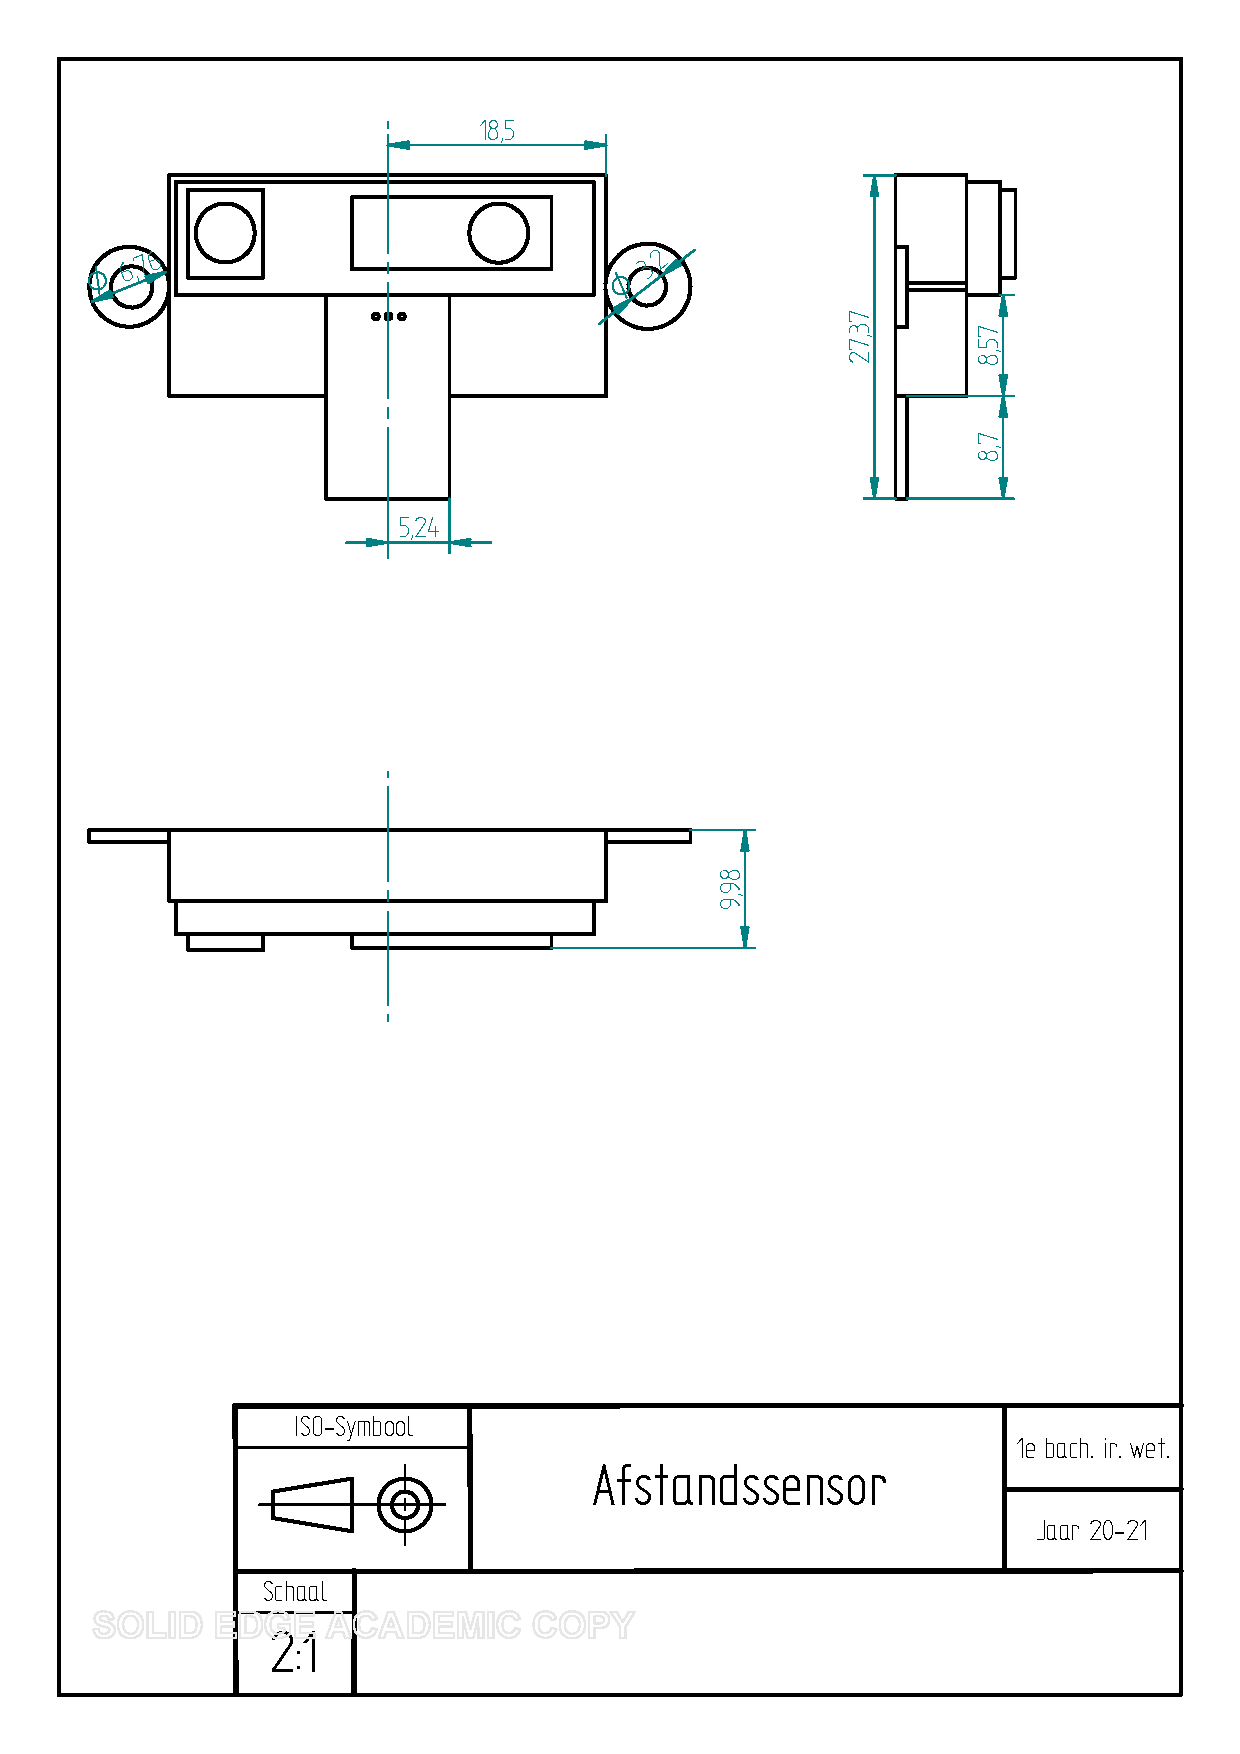
\includepdf{TechnischeTekeningAfstandssensor.pdf}\label{TechTekAfstandssensor}
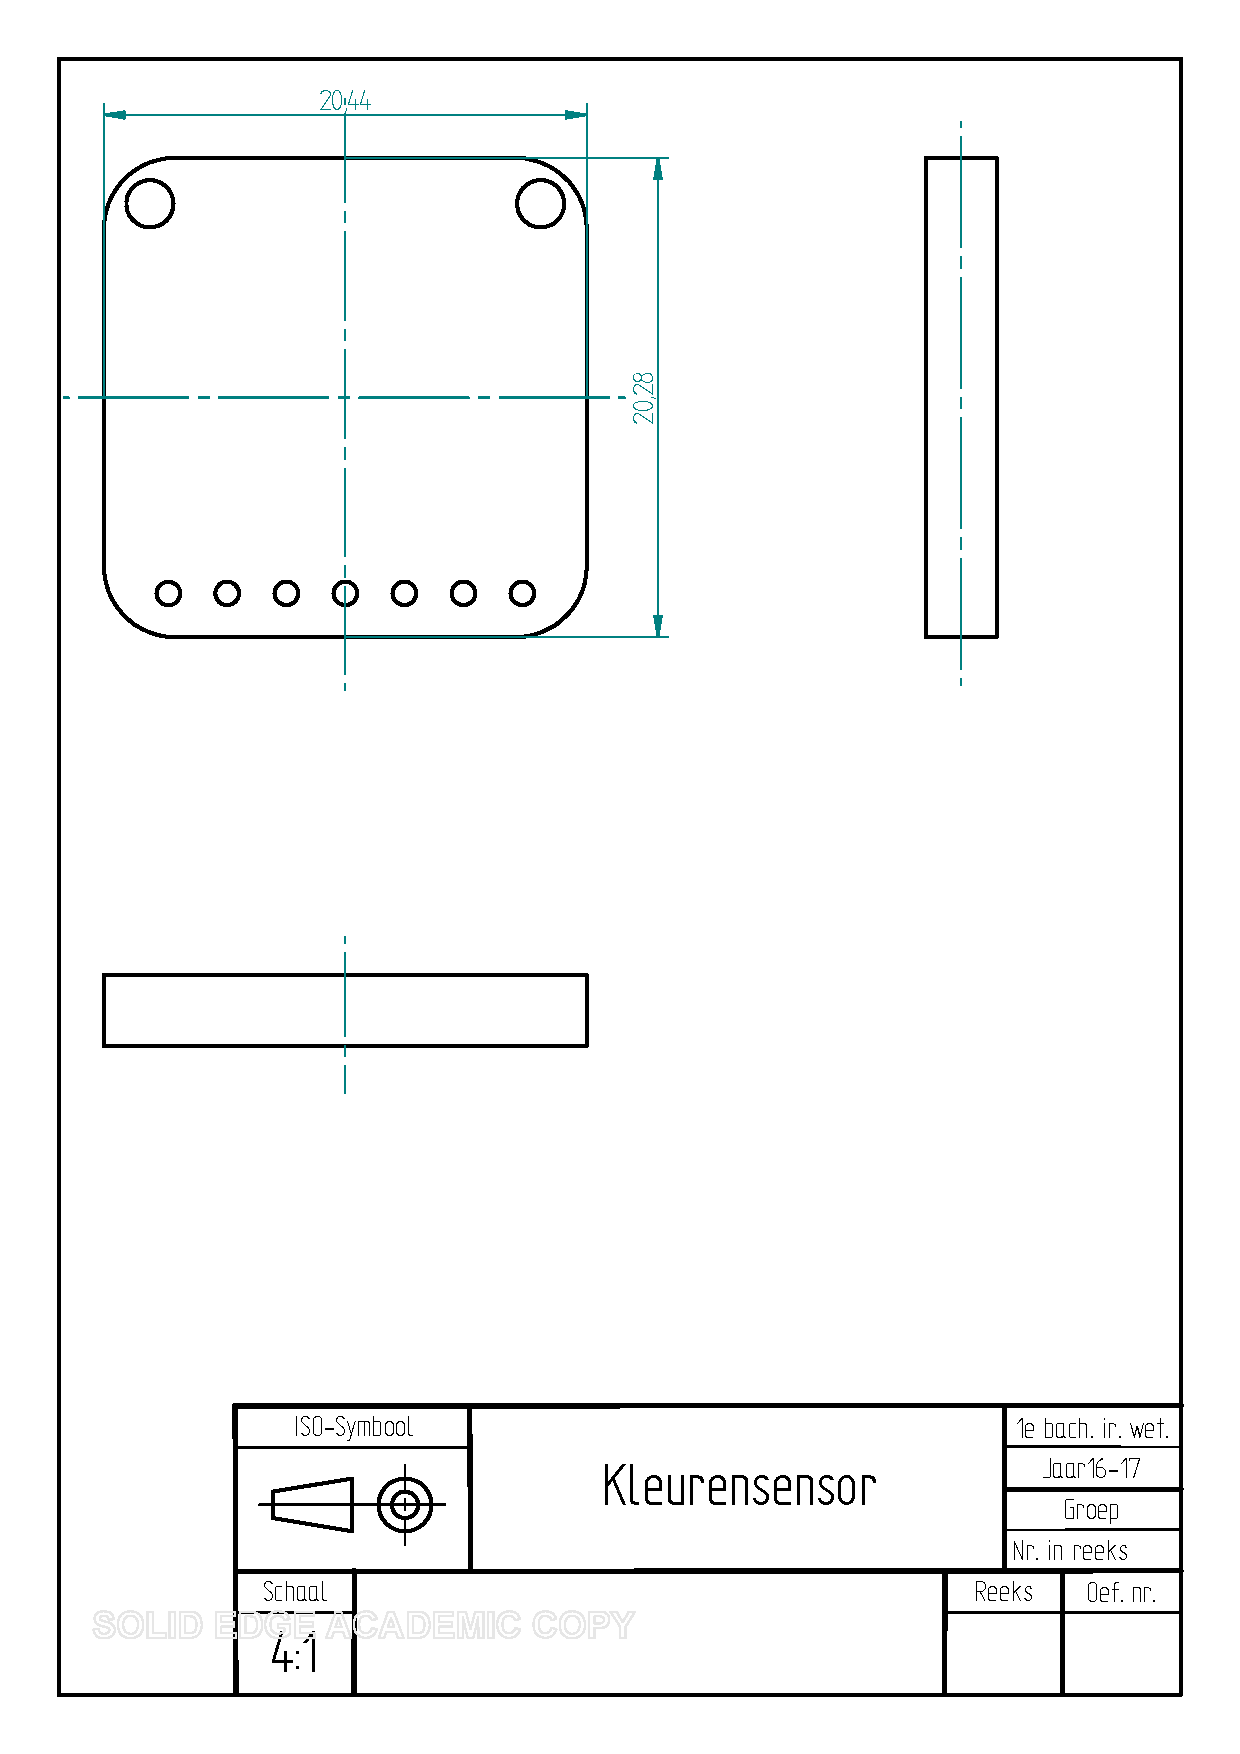
\includepdf{TechnischeTekeningKleurensensor.pdf}\label{TechTekKleurensensor}




\bibliographystyle{plain}
\bibliography{bronnen_verslag}
\bibliographystyle{unsrt}
\end{document}
